%!Tex Program = xelatex
%\documentclass[a4paper]{article}
\documentclass[a4paper]{ctexart}

\usepackage[utf8]{inputenc}%告诉 LaTeX TeX文档的输入(文件)编码(为utf-8)
\usepackage{amsmath}%数学公式相关
\usepackage{amssymb}%更多的数学符号
\usepackage{caption}%控制题目/说明文字的样式
\usepackage{graphicx, subfig}%插入图片
\usepackage{ctex}%中文宏包
\usepackage{float}%强行保留图片位置用
%\usepackage[T1]{fontenc}%可以调用各种编码字体,并可有多重选项,其中最后的选项将成为系统默认编码
%\usepackage{textcomp}%提供了许多 TS1 编码的可直接在文本中使用的常见数理单位和货币符号
\usepackage{url}%插入网址
\usepackage{hyperref}%超链接

\usepackage{tikz}%TiKZ绘图
\usetikzlibrary{arrows,shapes,chains}
\usetikzlibrary{graphs, positioning, quotes, shapes.geometric}
\usepackage{array}

\usepackage{listings}%更好看的代码
\usepackage{xltxtra}%listings中文支持
\usepackage{color}%listings字体颜色相关
\definecolor{dkgreen}{rgb}{0,0.6,0}
\definecolor{gray}{rgb}{0.5,0.5,0.5}
\definecolor{mauve}{rgb}{0.58,0,0.82}

\lstset{frame=tb,%listings代码区各种设置
	language=Python,
	aboveskip=3mm,
	belowskip=3mm,
	showstringspaces=false,
	columns=flexible,
	basicstyle={\small\ttfamily},
	numbers=left,%设置行号位置none不显示行号
	%numberstyle=\tiny\courier, %设置行号大小
	numberstyle=\tiny\color{gray},
	keywordstyle=\color{blue},
	commentstyle=\color{dkgreen},
	stringstyle=\color{mauve},
	breaklines=true,
	breakatwhitespace=true,
	escapeinside=``,%逃逸字符(1左面的键),用于显示中文例如在代码中`中文...`
	tabsize=4,
	extendedchars=false %解决代码跨页时,章节标题,页眉等汉字不显示的问题
}

\hypersetup{hypertex=true,%超链接设置
	colorlinks=true,
	linkcolor=blue,
	anchorcolor=blue,
	citecolor=blue}
%%%%%%%%%%%%%%%%%%%%%%%%%%%%%%%%%%%%%%%%%%%%%%%%%%%%%%%%%%%%%%%%%%%%%
%% Place any additional macros here.  Please use \newcommand* where
%% possible, and avoid layout-changing macros (which are not used
%% when typesetting).
%%%%%%%%%%%%%%%%%%%%%%%%%%%%%%%%%%%%%%%%%%%%%%%%%%%%%%%%%%%%%%%%%%%%%
%\newcommand*\mycommand[1]{\texttt{\emph{#1}}}

%\setmainfont[Mapping=tex-text]{AR PL UMing CN:style=Light}
%\setmainfont[Mapping=tex-text]{AR PL UKai CN:style=Book}
%\setmainfont[Mapping=tex-text]{WenQuanYi Zen Hei:style=Regular}
%\setmainfont[Mapping=tex-text]{WenQuanYi Zen Hei Sharp:style=Regular}
%\setmainfont[Mapping=tex-text]{AR PL KaitiM GB:style=Regular} 
%\setmainfont[Mapping=tex-text]{AR PL SungtiL GB:style=Regular} 
%\setmainfont[Mapping=tex-text]{WenQuanYi Zen Hei Mono:style=Regula}

\author{吴泓鹰\\数学与应用数学(强基计划)\quad3210101890}
\title{\textbf{Julia 集的分析和探索}}
%\date{}

\begin{document}
\maketitle

\begin{abstract}
	本文介绍了Julia集的数学理论,并得到其图像的生成算法,进而使用Python程序实现生成不同条件下的Julia集图像的程序,探索得到Julia集在数学中的特征性质以及美丽之处,此外还对Mandelbrot集与Julia集的关系进行了简单分析。
	%\centering%使得关键字居中
	%\textbf{关键词:}Julia集,Mandelbrot集,Python
\end{abstract}

\CTEXsetup[format={\Large\bfseries}]{section}
\section{引入:问题背景}
Julia集由法国数学家Gaston Julia\footnote{详见\href{https://en.wikipedia.org/wiki/Gaston_Julia。}{Gaston Julia}}发现并命名,其是在复平面上构成分形点的集合。在复动力系统\footnote{一个数学分支,详见\href{https://en.wikipedia.org/wiki/Complex_dynamics}{Complex dynamics}。}的背景下,Julia集由使得任意小的扰动就会使迭代函数序列发生剧烈变化的值组成,这体现了Julia集行为上的混沌性\footnote{混沌理论相关,详见\href{https://en.wikipedia.org/wiki/Chaos_theory}{Chaos teory}。}。关于Julia集有很多有趣和美丽的地方,下面将对Julia集进行简单的分析和探索。\cite{julia_wiki}

\section{分析:生成Julia集}

\subsection{数学理论}
Julia集一般可以定义为使得复函数$f_c(z)=z^2+c$经过无数次迭代后能够不发散的复数$z$的集合,其中$c\in\mathbb{C}$,我们一般取$|c|<2$。\cite{julia_Ju}

进一步的,令$f(z)$为有理函数,其定义为$\displaystyle f(z):=\frac{p(z)}{q(z)}$,其中$z\in\mathbb{C}^*,\mathbb{C}^*$为黎曼球面$\mathbb{C}\bigcup\{\infty\}$,$p,q$为没有公因式的多项式。则拓展后的Julia集$J_R$为在经过无数次$f(z)$迭代后不发散的$z$的集合,而真正的Julia集$J$为$J_R$的边界$\partial J_R$。\cite{julia_wolfram}

\subsection{算法实现}
为了在计算机上生成Julia集的图像,我们首先需要一个算法来实现这一过程。考虑到计算机能够处理的迭代次数是有限的,因此我们把“不发散”理解为“$|z|<2$”,并且每经过一次迭代,我们将其中“不发散”点的颜色改变一点,“发散”点则保留其原来的颜色,这样我们就能清晰地观察到生成图像的特征。具体算法的流程图如下:\cite{julia_zhihuRe}\cite{mandelbrotsetpython}
\begin{figure}[H]
\tikzstyle{io} = [trapezium, trapezium left angle = 60, trapezium right angle = 120, minimum width = 1cm, text centered, draw = black, fill = white, align=center]
\centering
\begin{tikzpicture}[node distance=10pt]
	\node[draw, rounded corners](start){开始};
	\node[draw, below=of start](step 1){设置坐标系长宽$a,b$与$i=0$};
	\node[draw, below=of step 1](step 2){设置每个像素占长宽$d$};
	\node[draw, below=25pt of step 2](step 3){取每个像素的复值$z$};
	\node[draw, io, right=20pt of step 2](input){输入复常数$c$\\与迭代次数$N$};
	\node[draw, diamond, aspect=2, below=of input] (choice 1) {$|z|<2$};
	\node[draw, diamond, aspect=2, below=of choice 1] (choice 2) {$i<N$};
	\node[draw, below=30pt of step 3] (step 4) {$z=f(z),i=i+1$};
	\node[draw, right=of choice 2] (step 5) {对该像素赋$i$对应的颜色};
	\node[draw, below=18pt of step 5] (step 6) {设置图片$dpi$};
	\node[draw, io , left=30pt of step 6] (step 7) {输出\texttt{.png}图片};
	\node[draw, rounded corners, below=18pt of step 4] (end) {结束};
	
	\draw[->] (choice 1) --node[above] {否} (choice 1 -|step 5) -> (step 5);
	\graph{
		(start) -> (step 1) -> (step 2) -> (input) -> (choice 1) -> ["是"left](choice 2) ->["是"above](step 4) -> (choice 1);
		(step 2) ->["取遍每个像素"left] (step 3) -> (choice 1);
		(choice 2) ->["否"above](step 5) -> (step 6) -> (step 7) -> (end);
	};
\end{tikzpicture}
\caption{Junia集图像生成的算法流程图}
\label{tu1}
\end{figure}

具体而言,为了实现该算法,我使用了Python编程语言进行程序设计\footnote{源代码见\href{run:./src/}{src}目录下的文件。},其中使用了库\verb|numpy|与\verb|matplotlib|,并且添加了一些细节,使用ipython3编译得到各式各样的Junia集的图像。

\section{探索:不同条件下的Julia集}
以下的所有数值算例均使用\verb|matplotlib|库中的\verb|imshow|函数生成,并且一般而言,我们取$f(z)=z^2+c$。设置的部分参数\footnote{以下生成的图片均根据标清参数生成,高清图片可到\href{run:./png/}{png}目录下查阅。}如下:
\begin{table}[htbp]
	\centering
	\begin{tabular}{|c|c|c|c|c|c|c|c|c|c|}
		\hline
		标清 & $a$ & $b$ & $d$ & $dpi$ & 高清 & $a$ & $b$ & $d$ & $dpi$ \\
		\hline
		 &$3.0$ & $3.0$ & $0.003$ & $300$ & & $3.0$ & $3.0$ & $0.001$ & $600$ \\
		\hline 
	\end{tabular}
\end{table}

\subsection{改变迭代次数$N$}
取$c=-0.4+0.6i$\cite{julia_wiki},再分别取$N=20,50,100,200$,如图\ref{tu2}所示。可以观察到:随着迭代次数的增加,Julia集的图像的精细程度越来越高,同时也体现出了更明显的自相似性。
\begin{figure}[H]
	\centering
	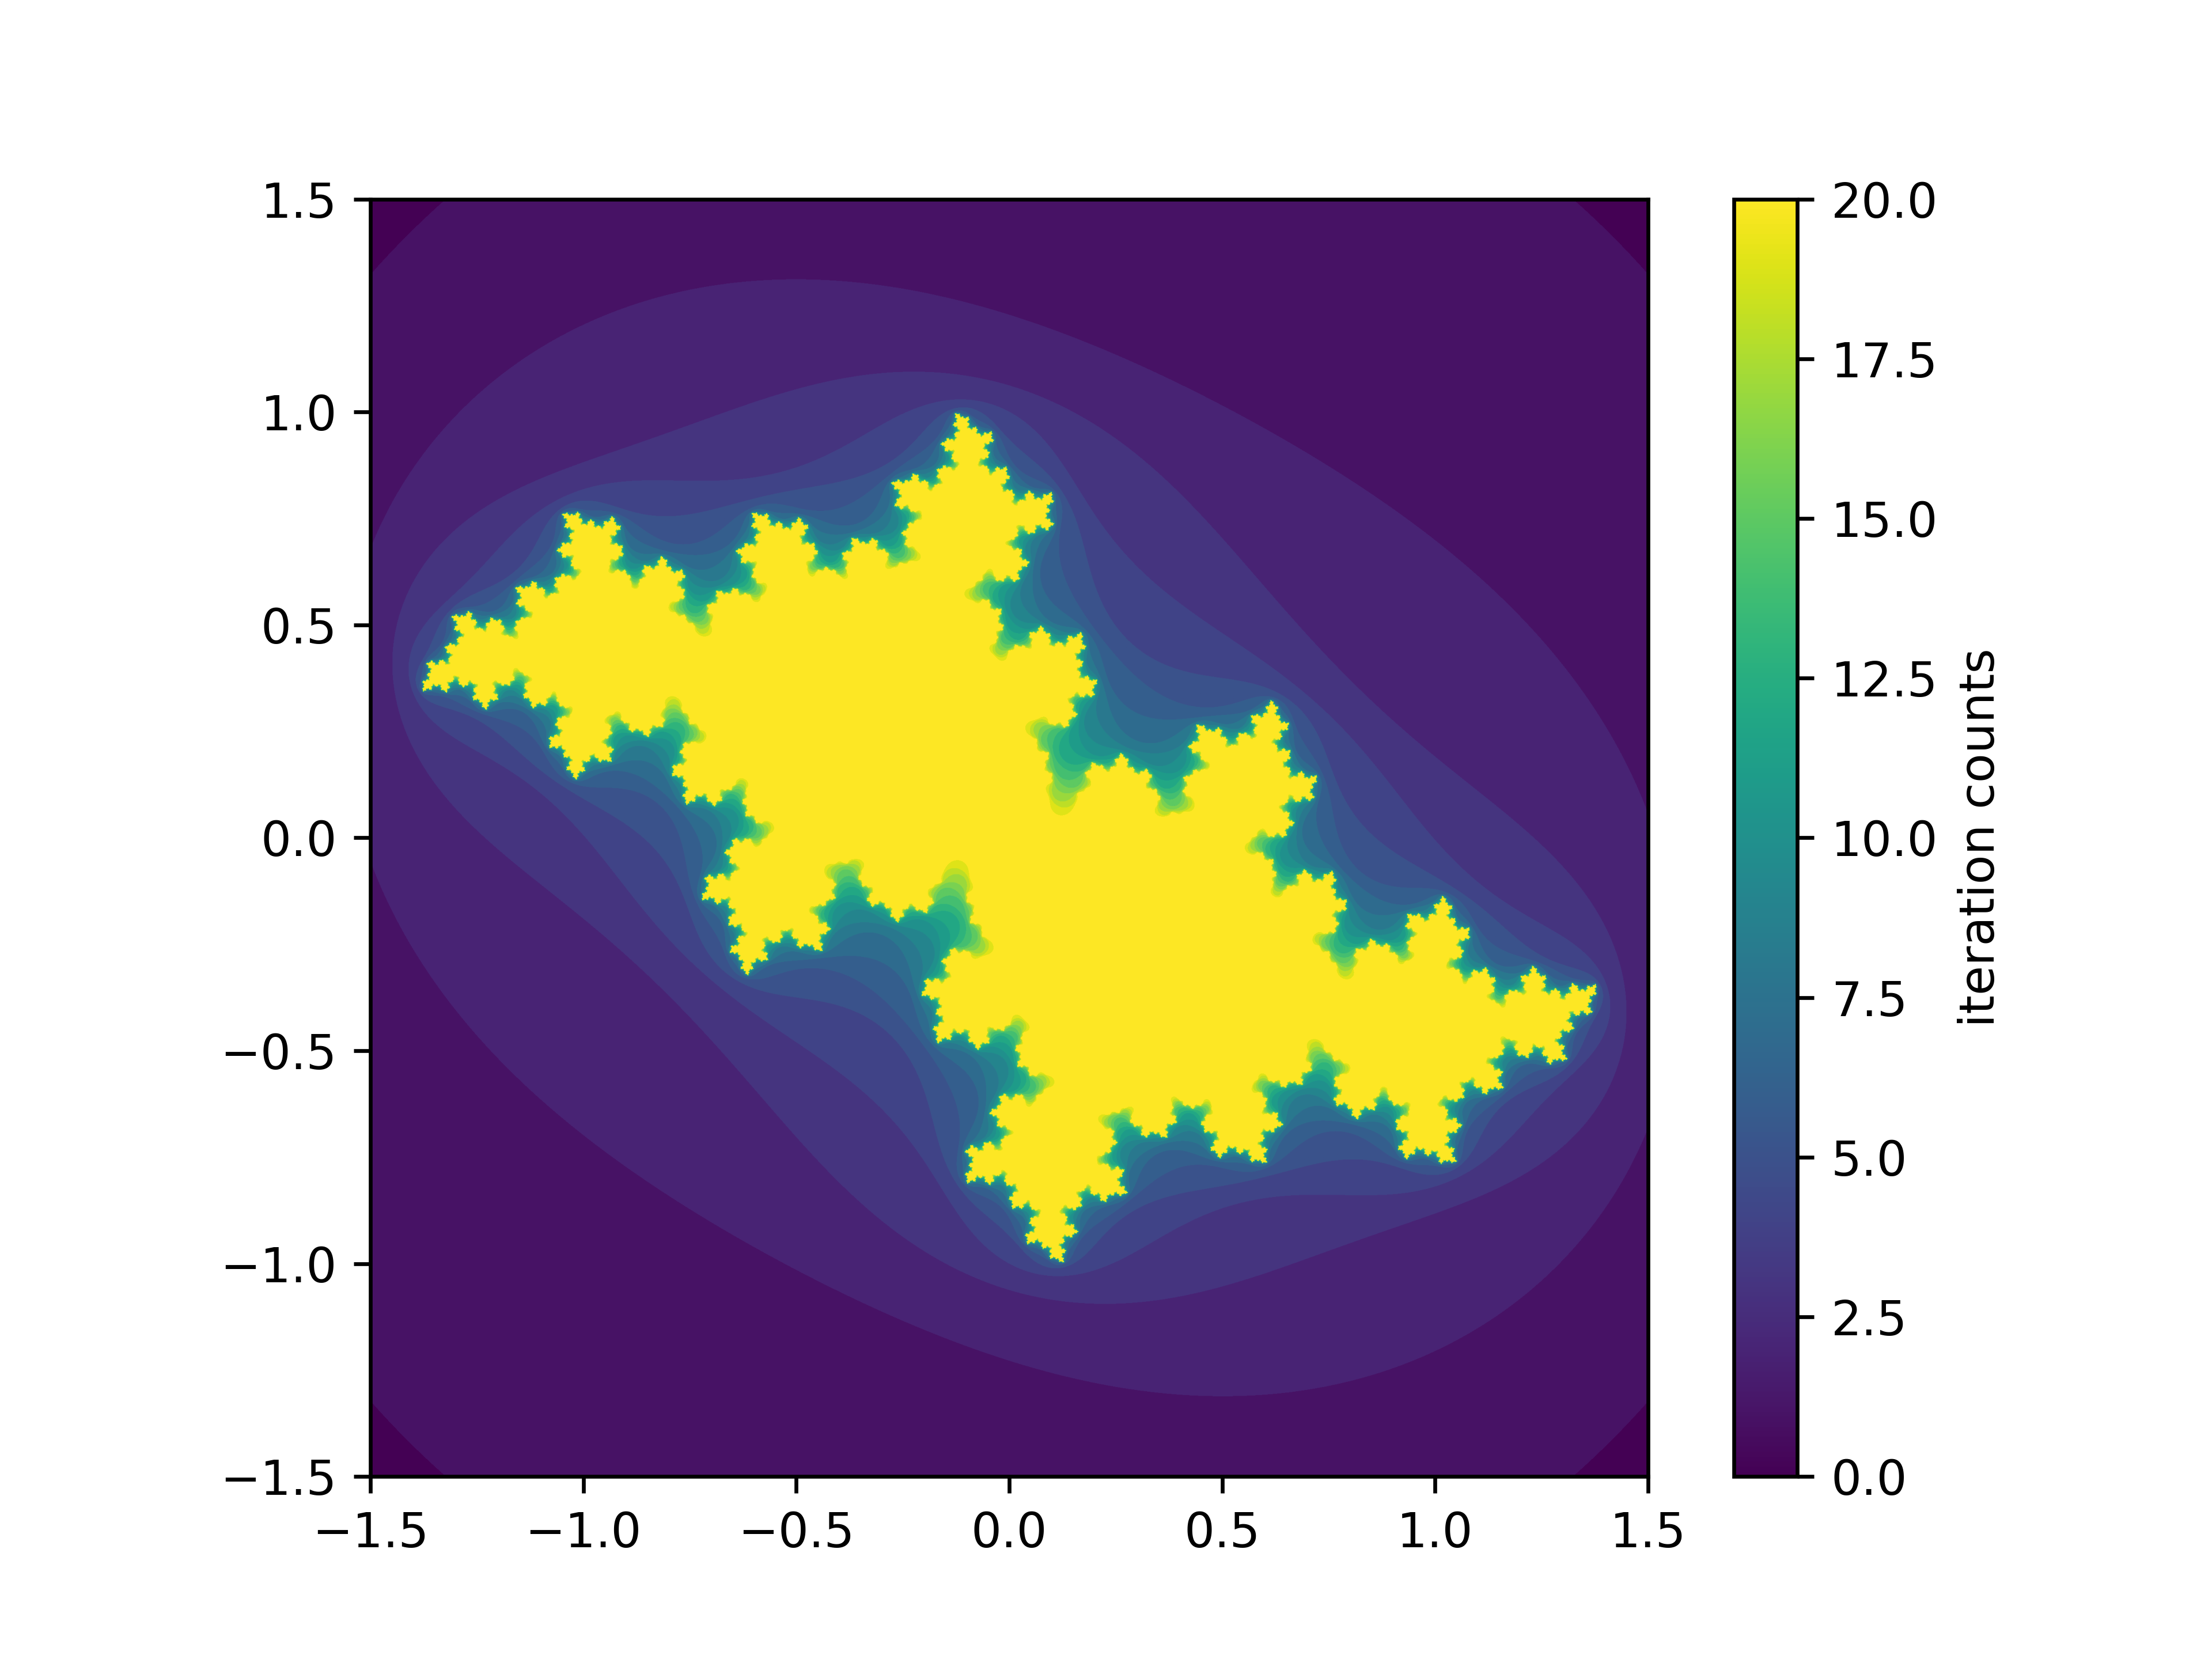
\includegraphics[width=.45\textwidth]{./png/300dpi/julia_cx-0.4cy0.6_N20.png}
	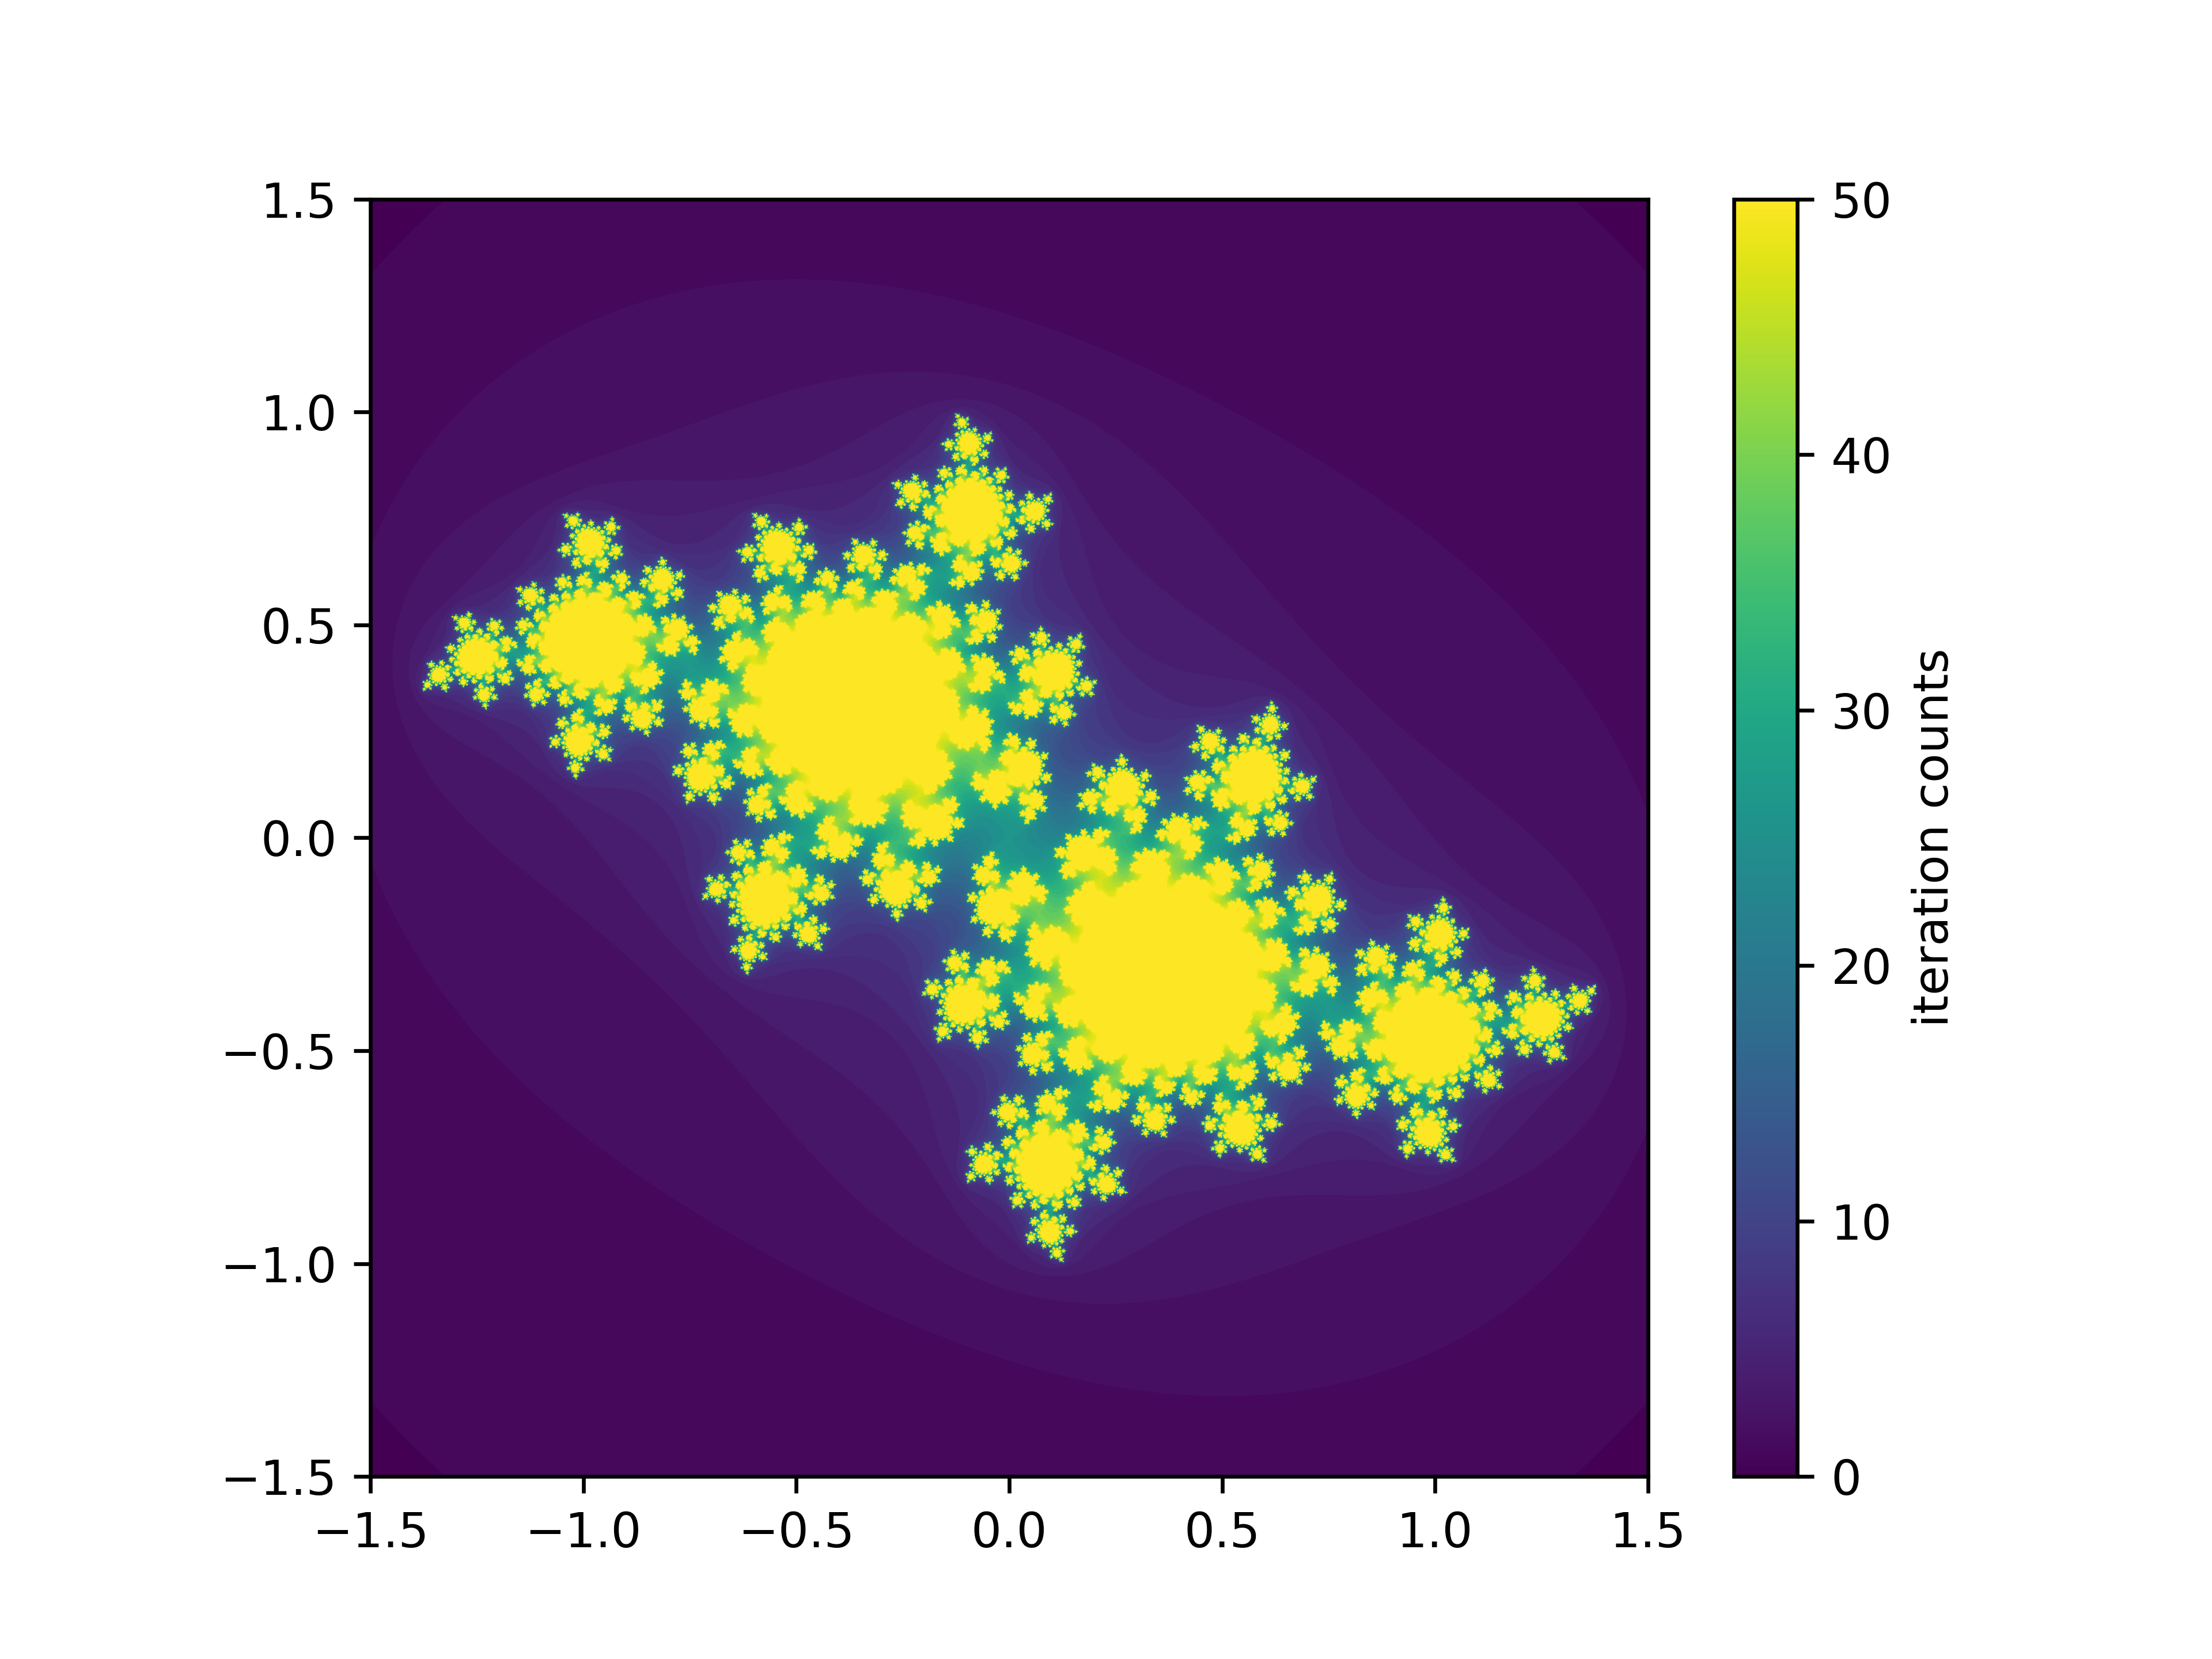
\includegraphics[width=.45\textwidth]{./png/300dpi/julia_cx-0.4cy0.6_N50.png}
	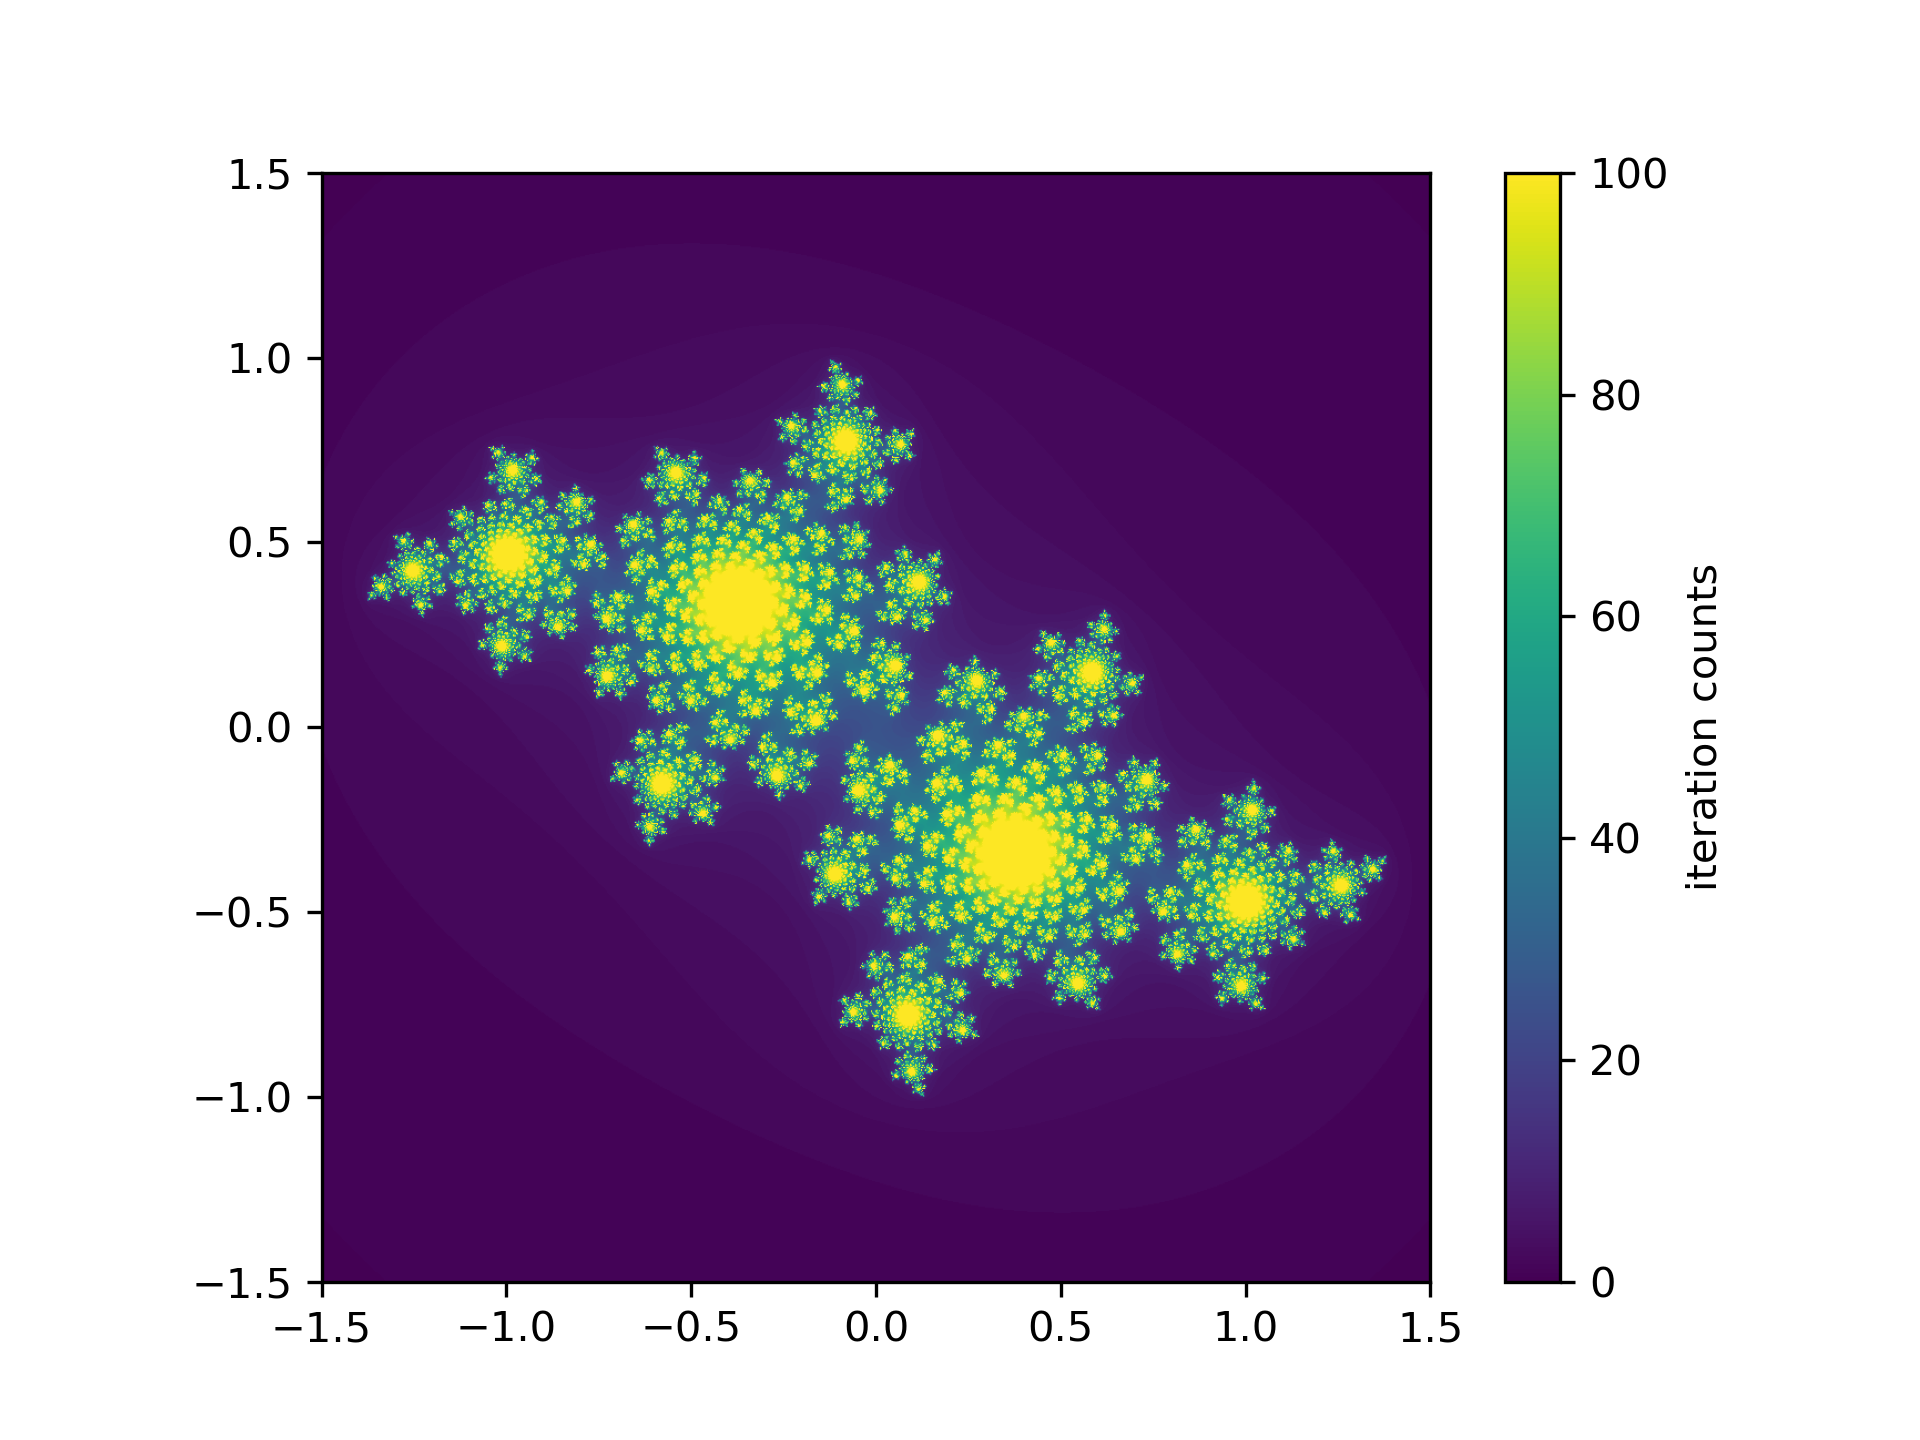
\includegraphics[width=.45\textwidth]{./png/300dpi/julia_cx-0.4cy0.6_N100.png}
	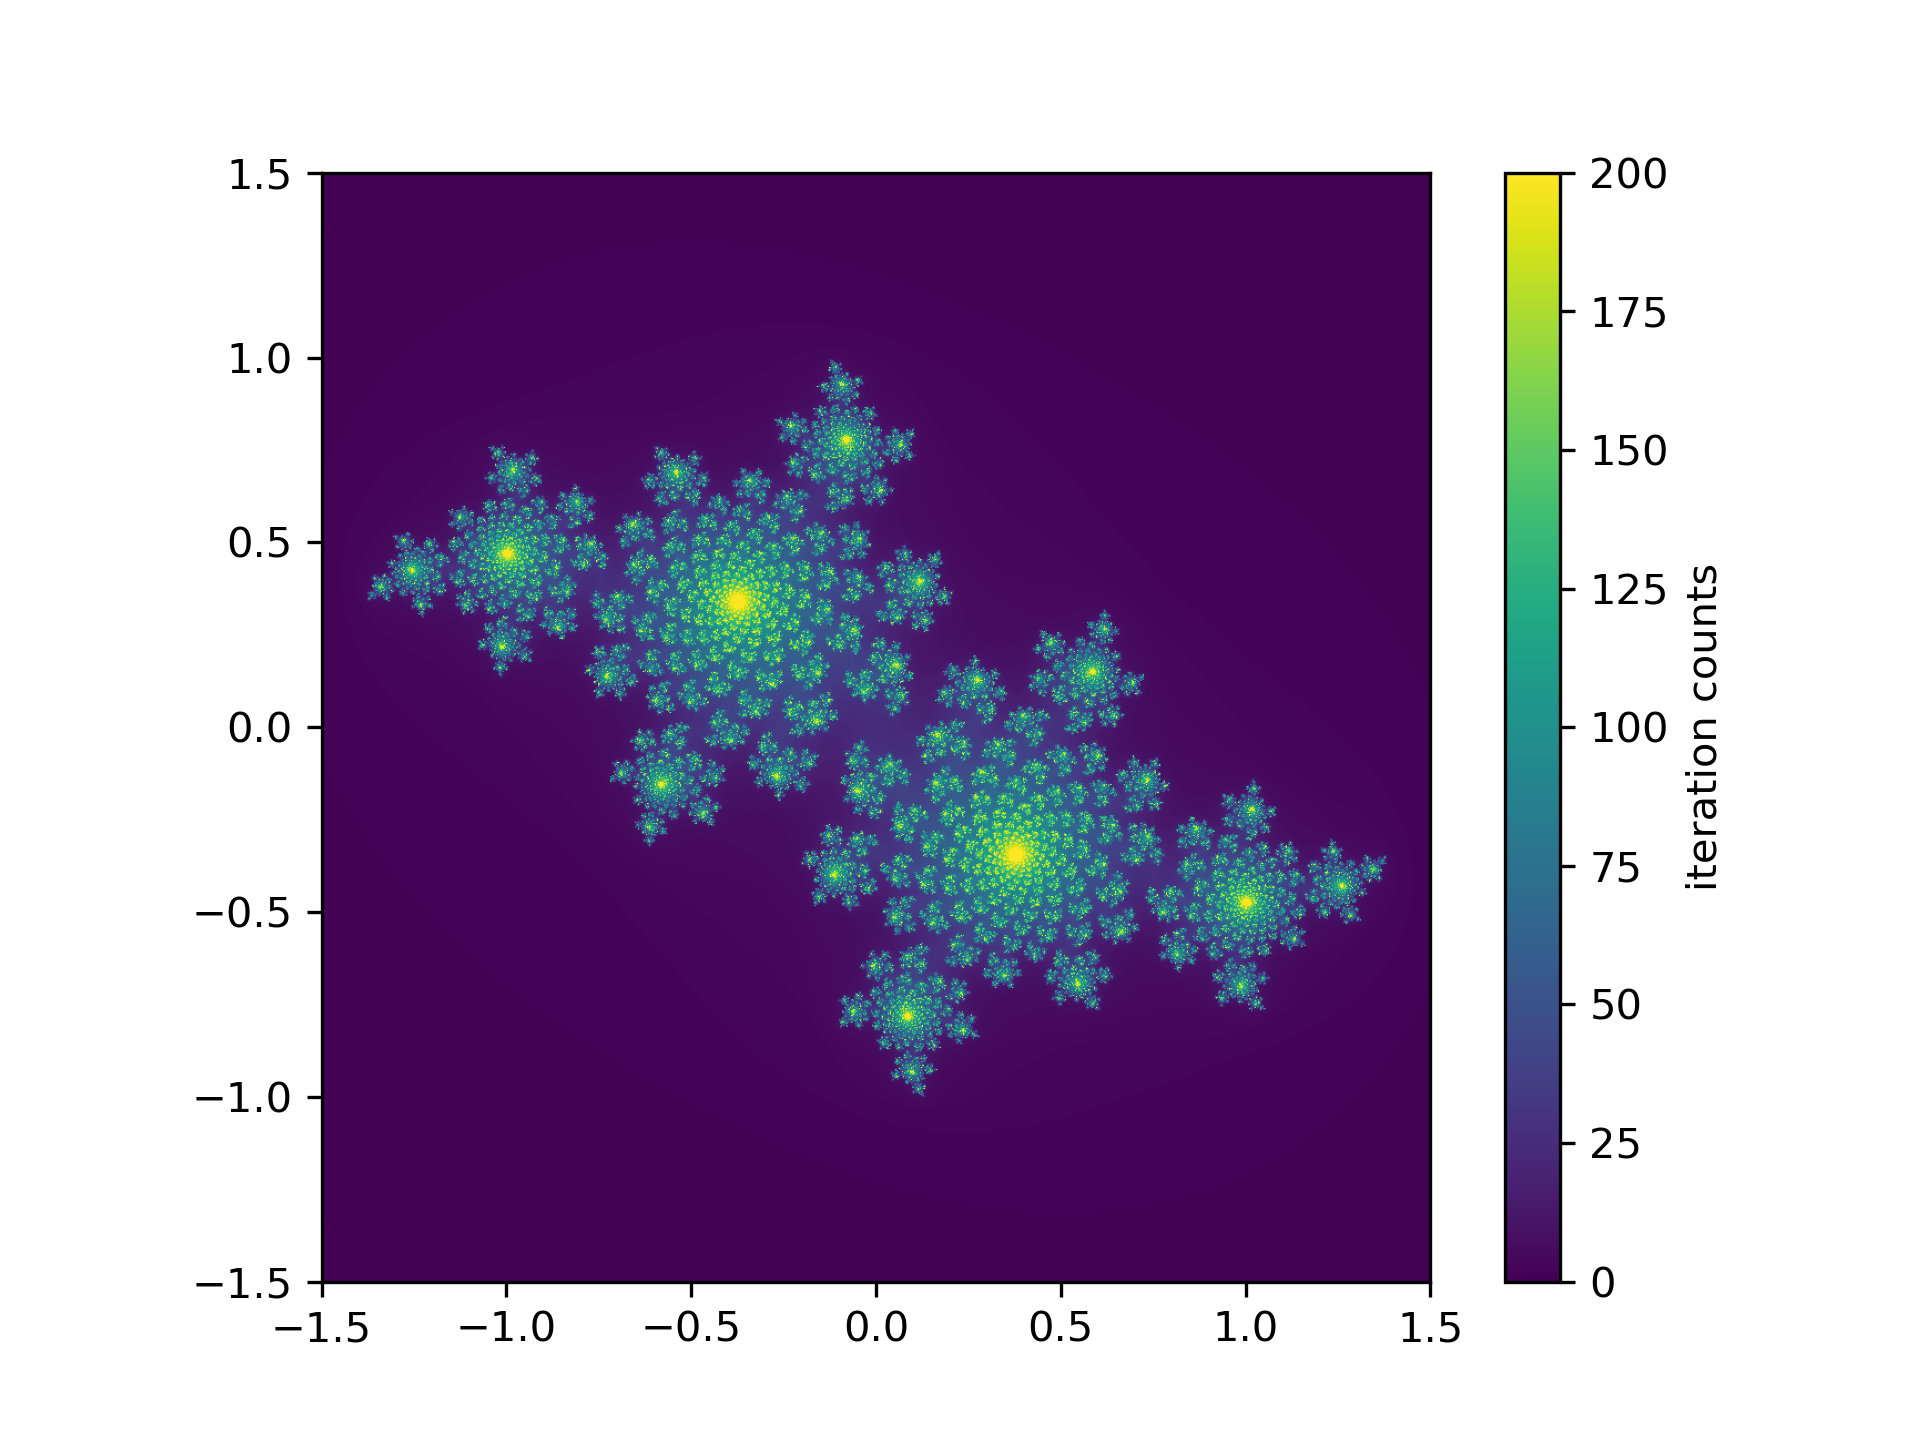
\includegraphics[width=.45\textwidth]{./png/300dpi/julia_cx-0.4cy0.6_N200.png}
	\caption{$c=-0.4+0.6i,N=20,50,100,200$}
	\label{tu2}
\end{figure}

\subsection{改变复常数$c$}
取$N=100$,再分别取$c_1=-0.4+0.6i,c_2=-0.8i,c_3=0.285+0.01i,c_4=-0.8+0.156i$\cite{julia_wiki},如图\ref{tu3}所示。可以观察到,对于不同的$c$值而言,Julia集的图像差异极大,这正体现了前文中所提到的Julia集具有的“混沌”性质;同时无论$c$值如何变化,得到的图像总是自相似且对称的,这也是为什么我们还会将Julia集描述为复平面上分形点的集合的原因。
\begin{figure}[H]
	\centering
	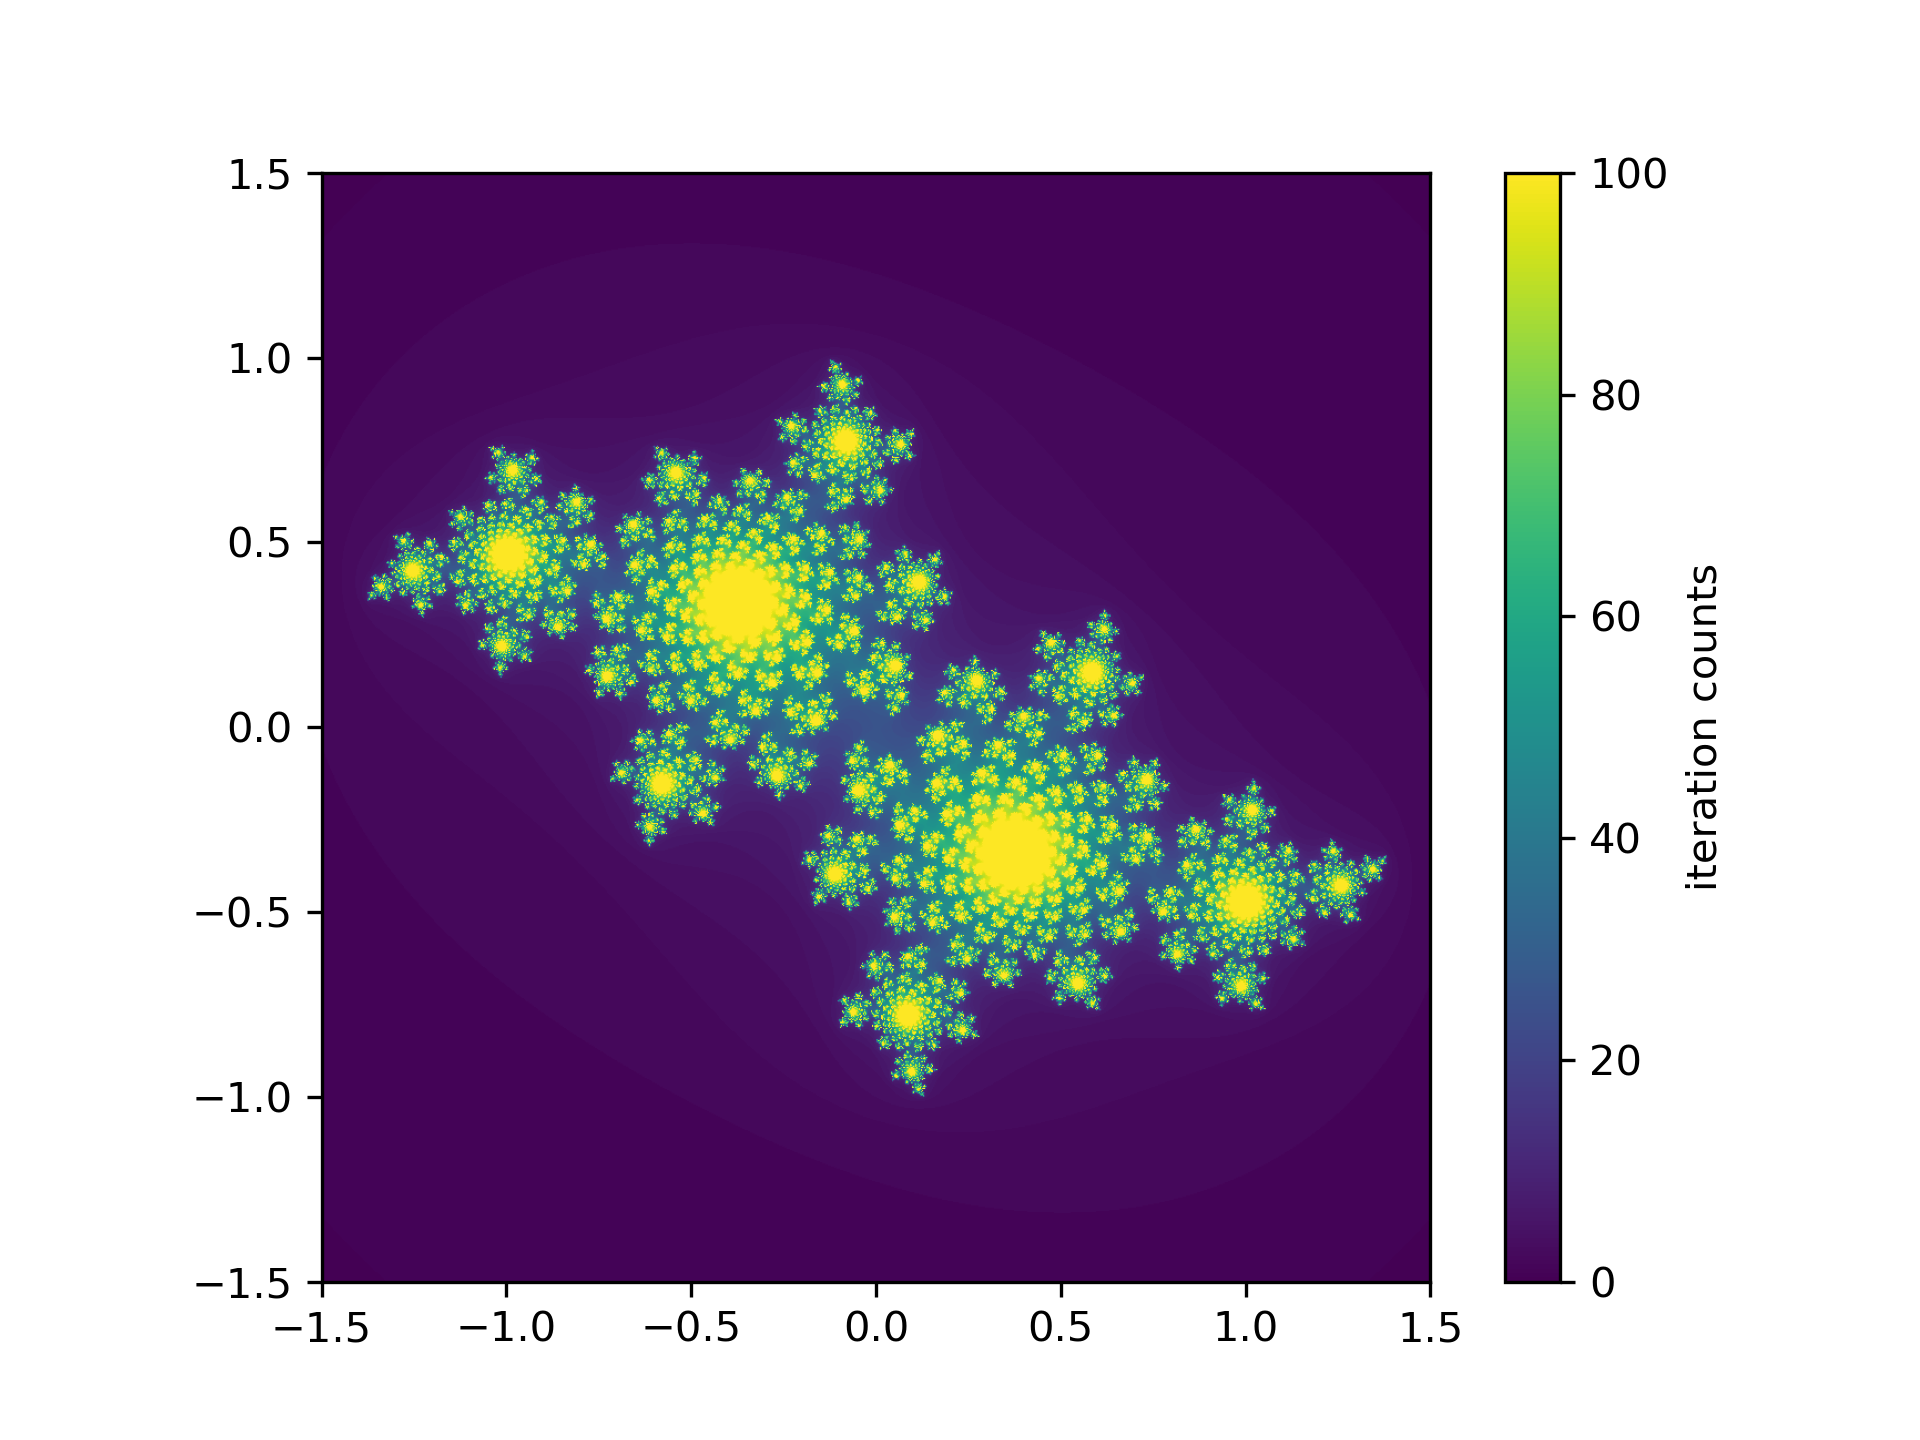
\includegraphics[width=.45\textwidth]{./png/300dpi/julia_cx-0.4cy0.6_N100.png}
	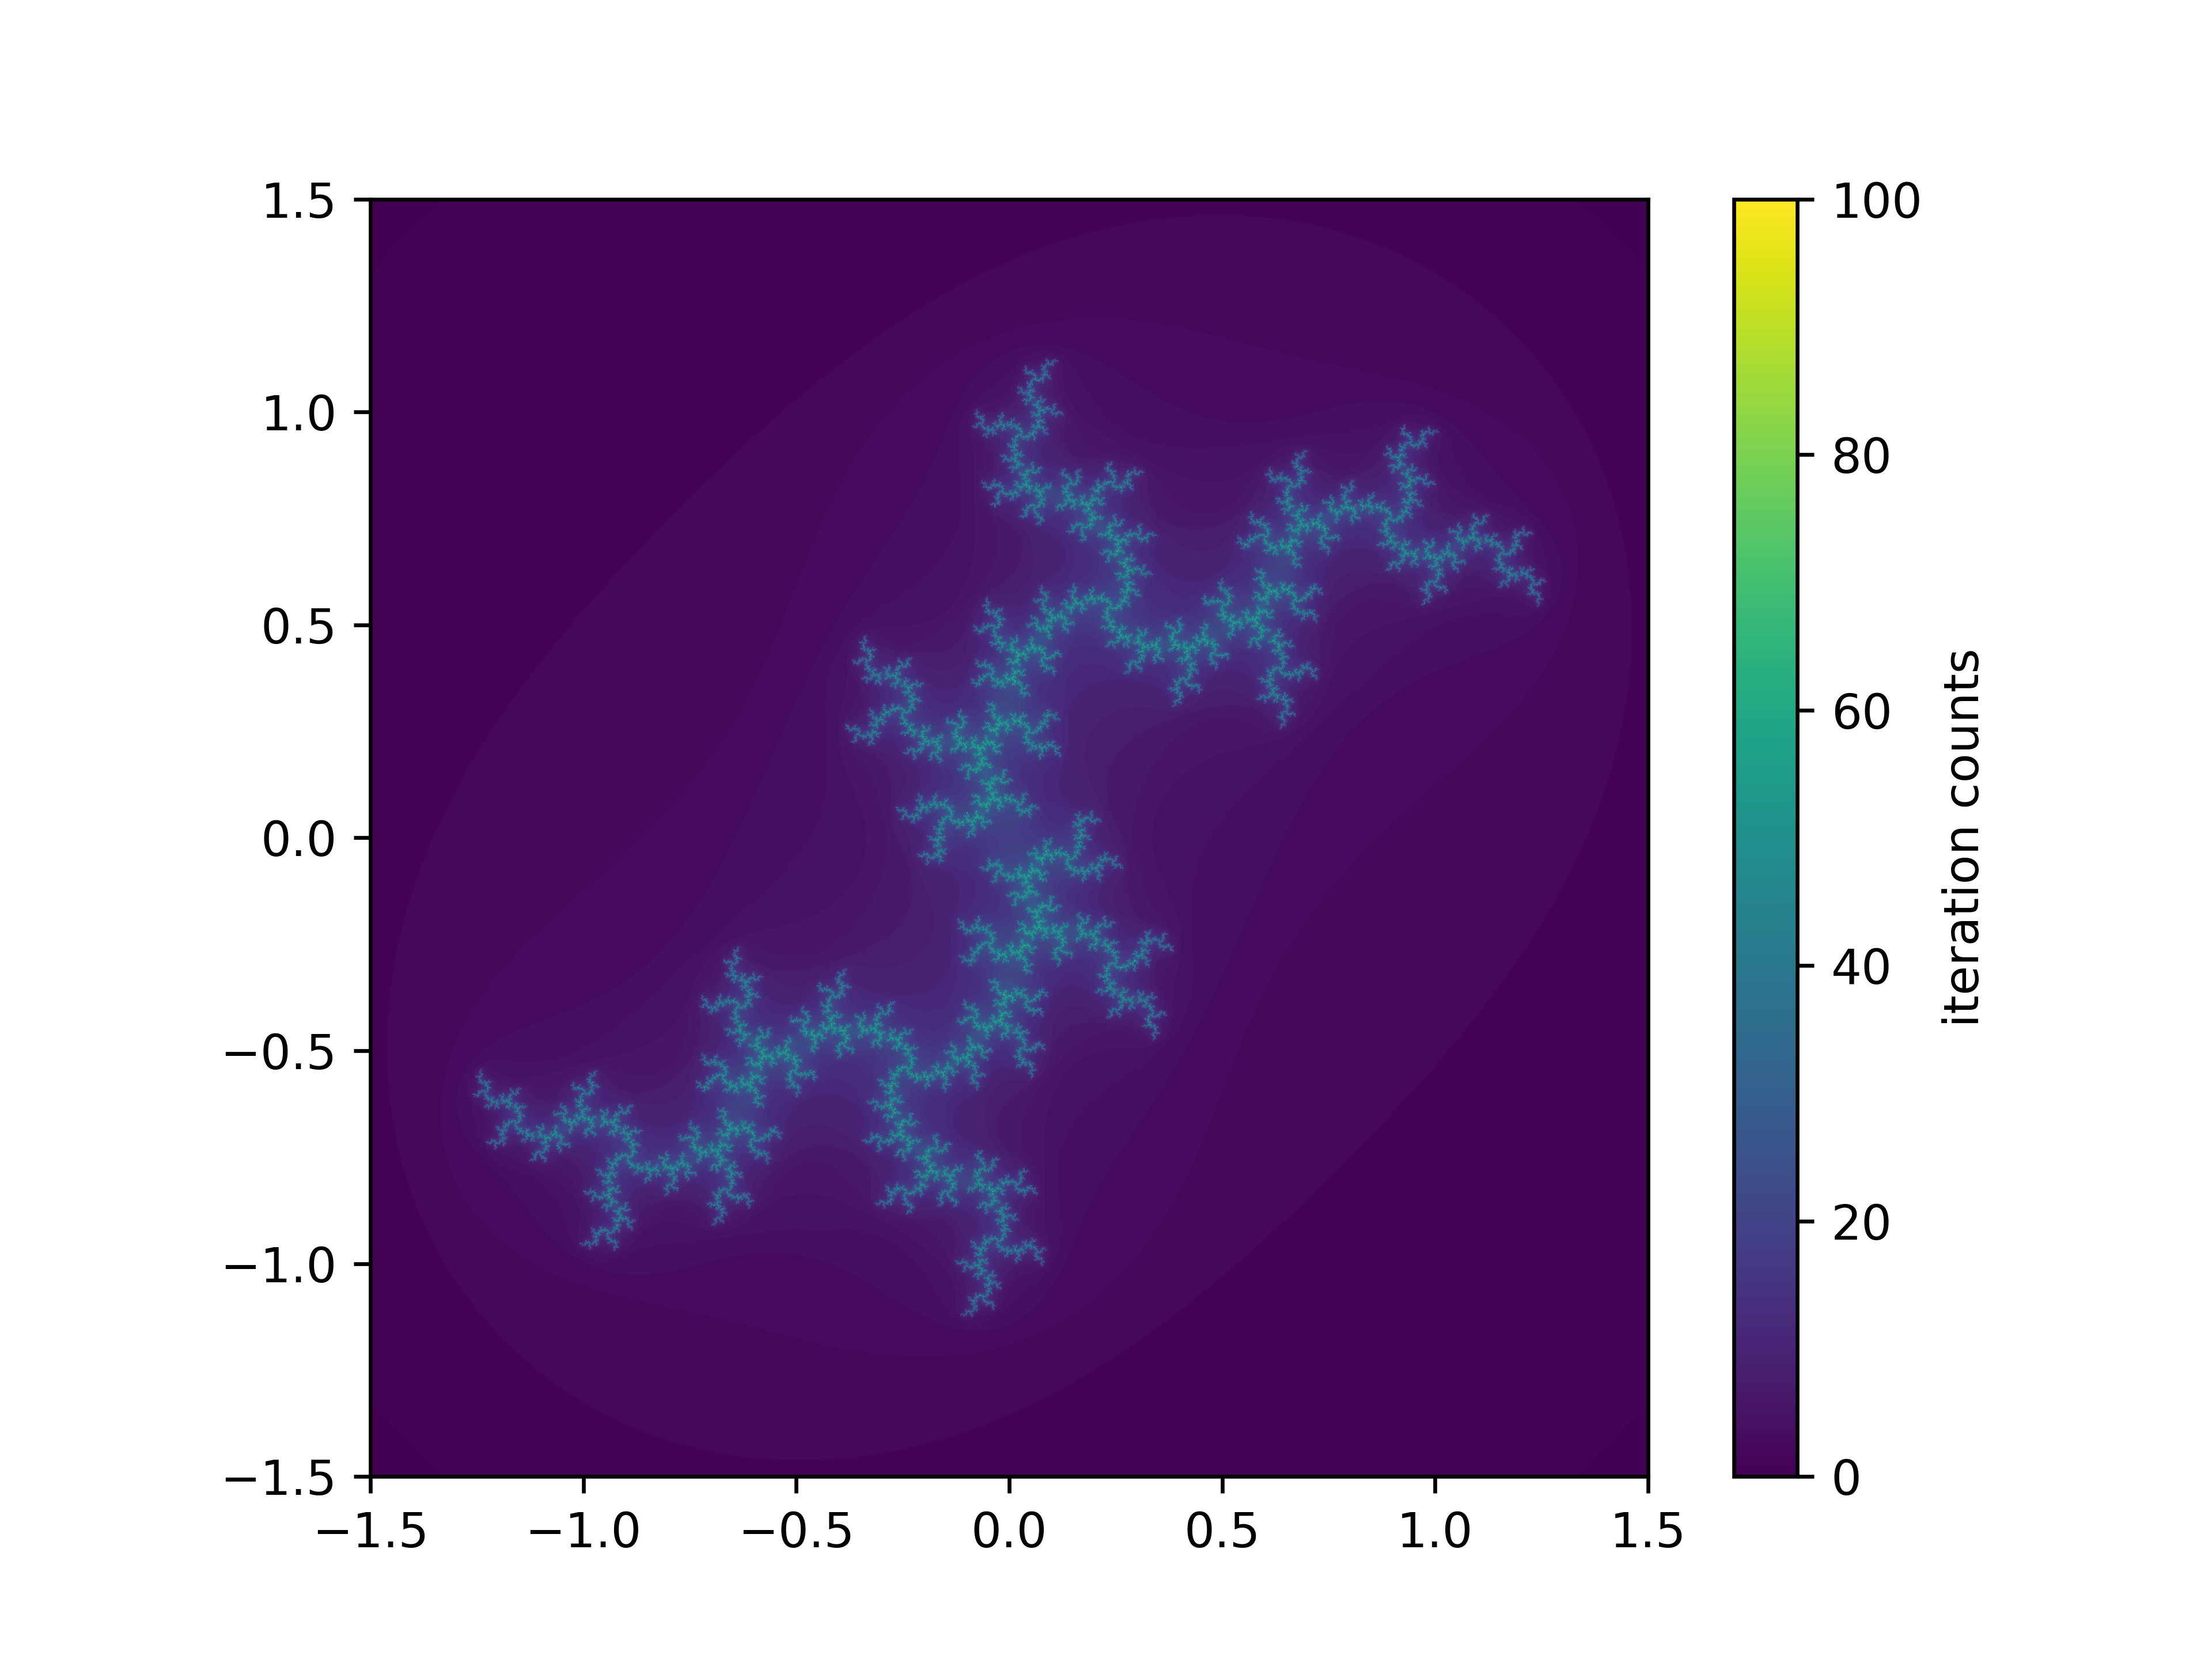
\includegraphics[width=.45\textwidth]{./png/300dpi/julia_cx0cy-0.8_N100.png}
\end{figure}
\begin{figure}[H]
	\centering
	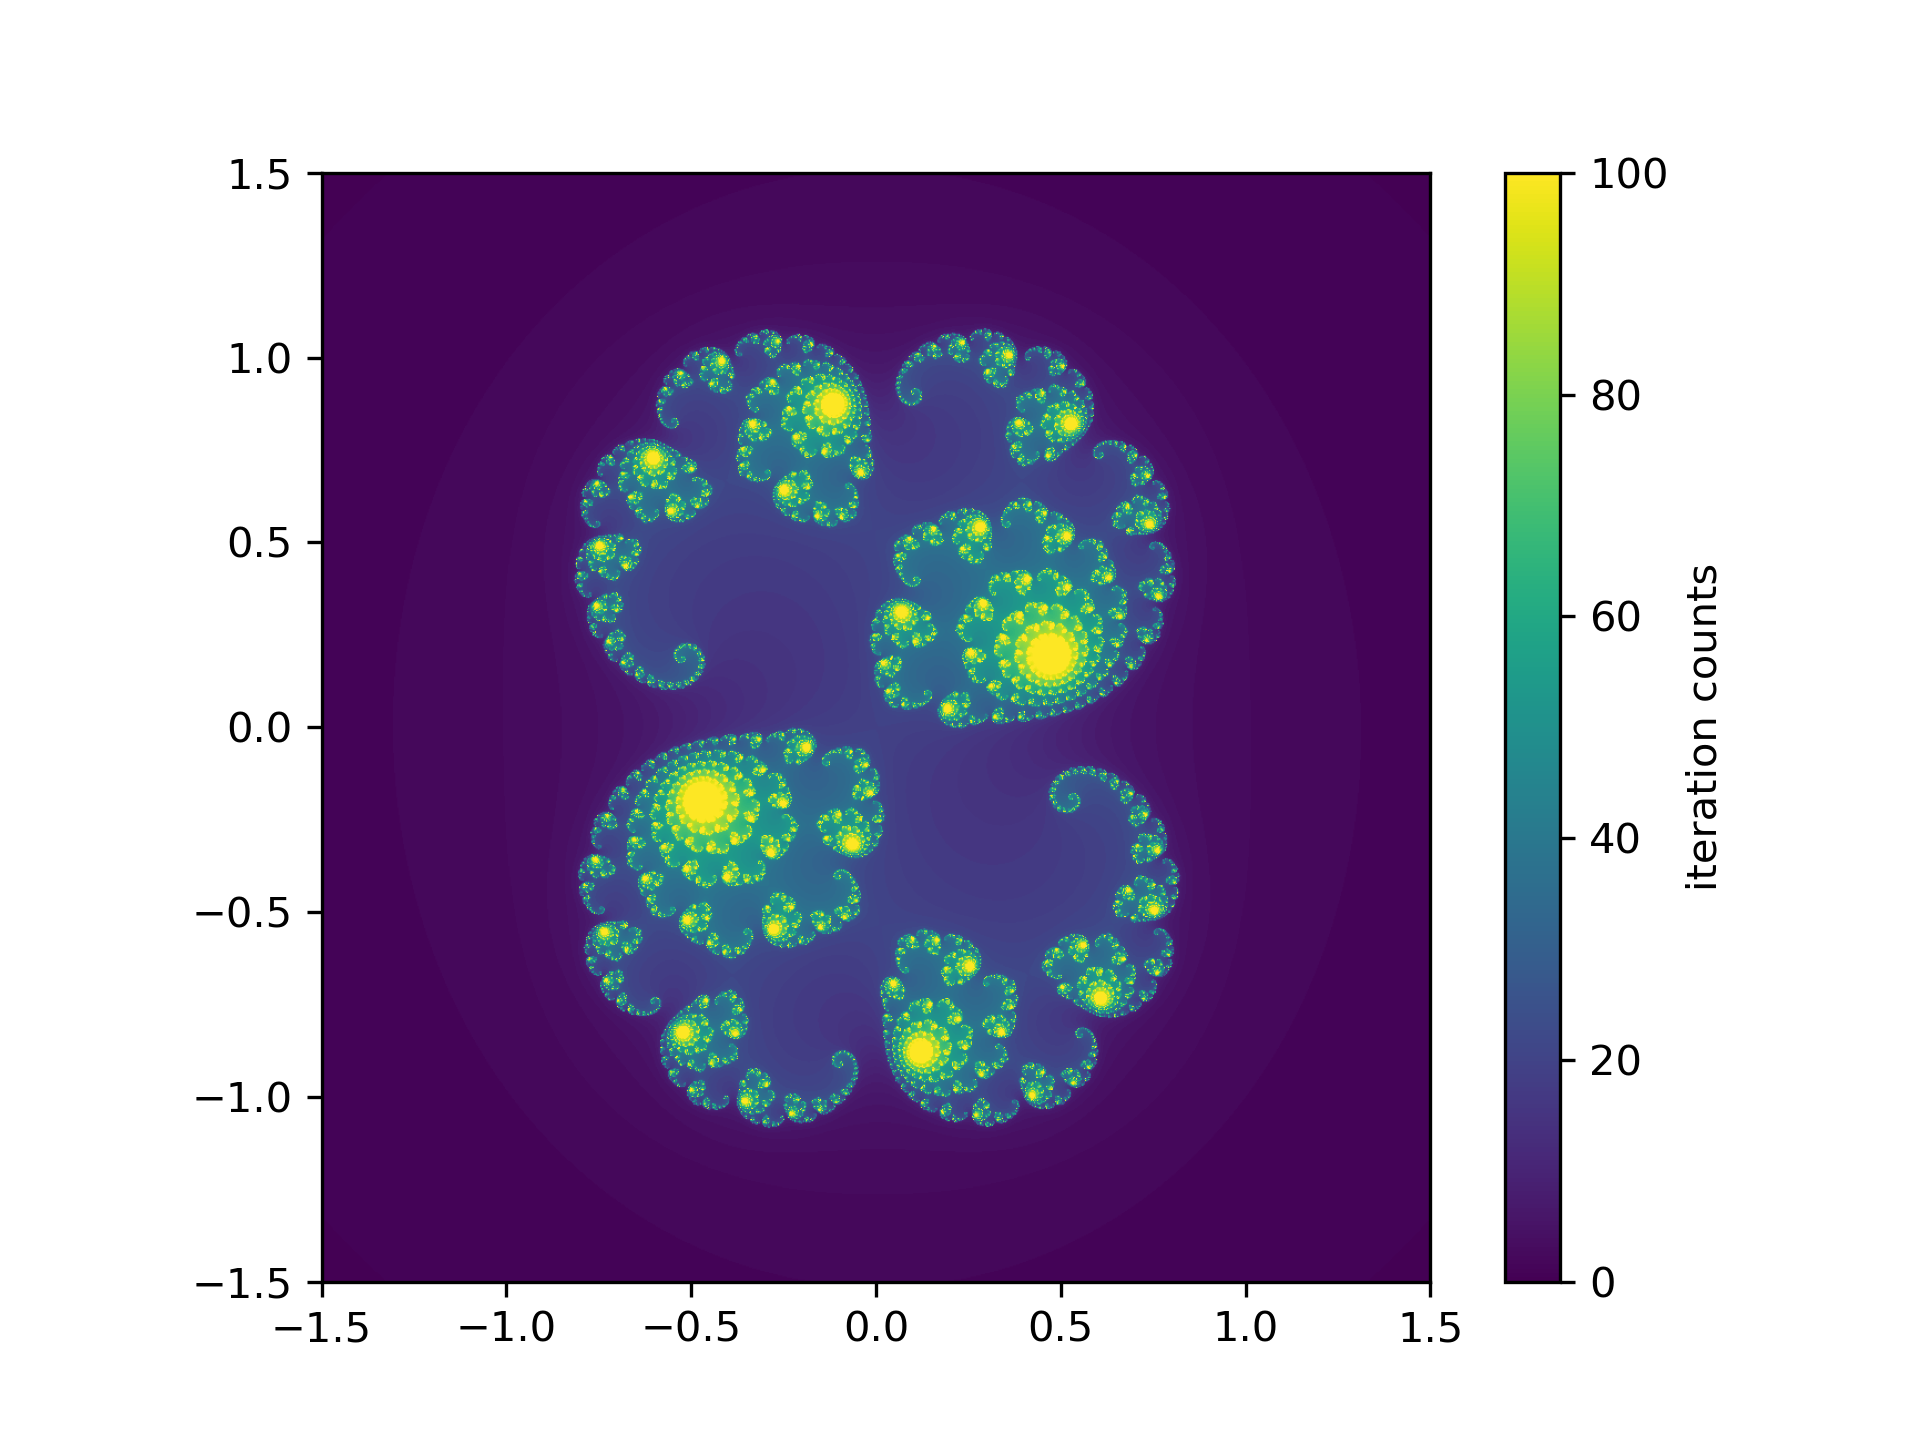
\includegraphics[width=.45\textwidth]{./png/300dpi/julia_cx0.285cy0.01_N100.png}
	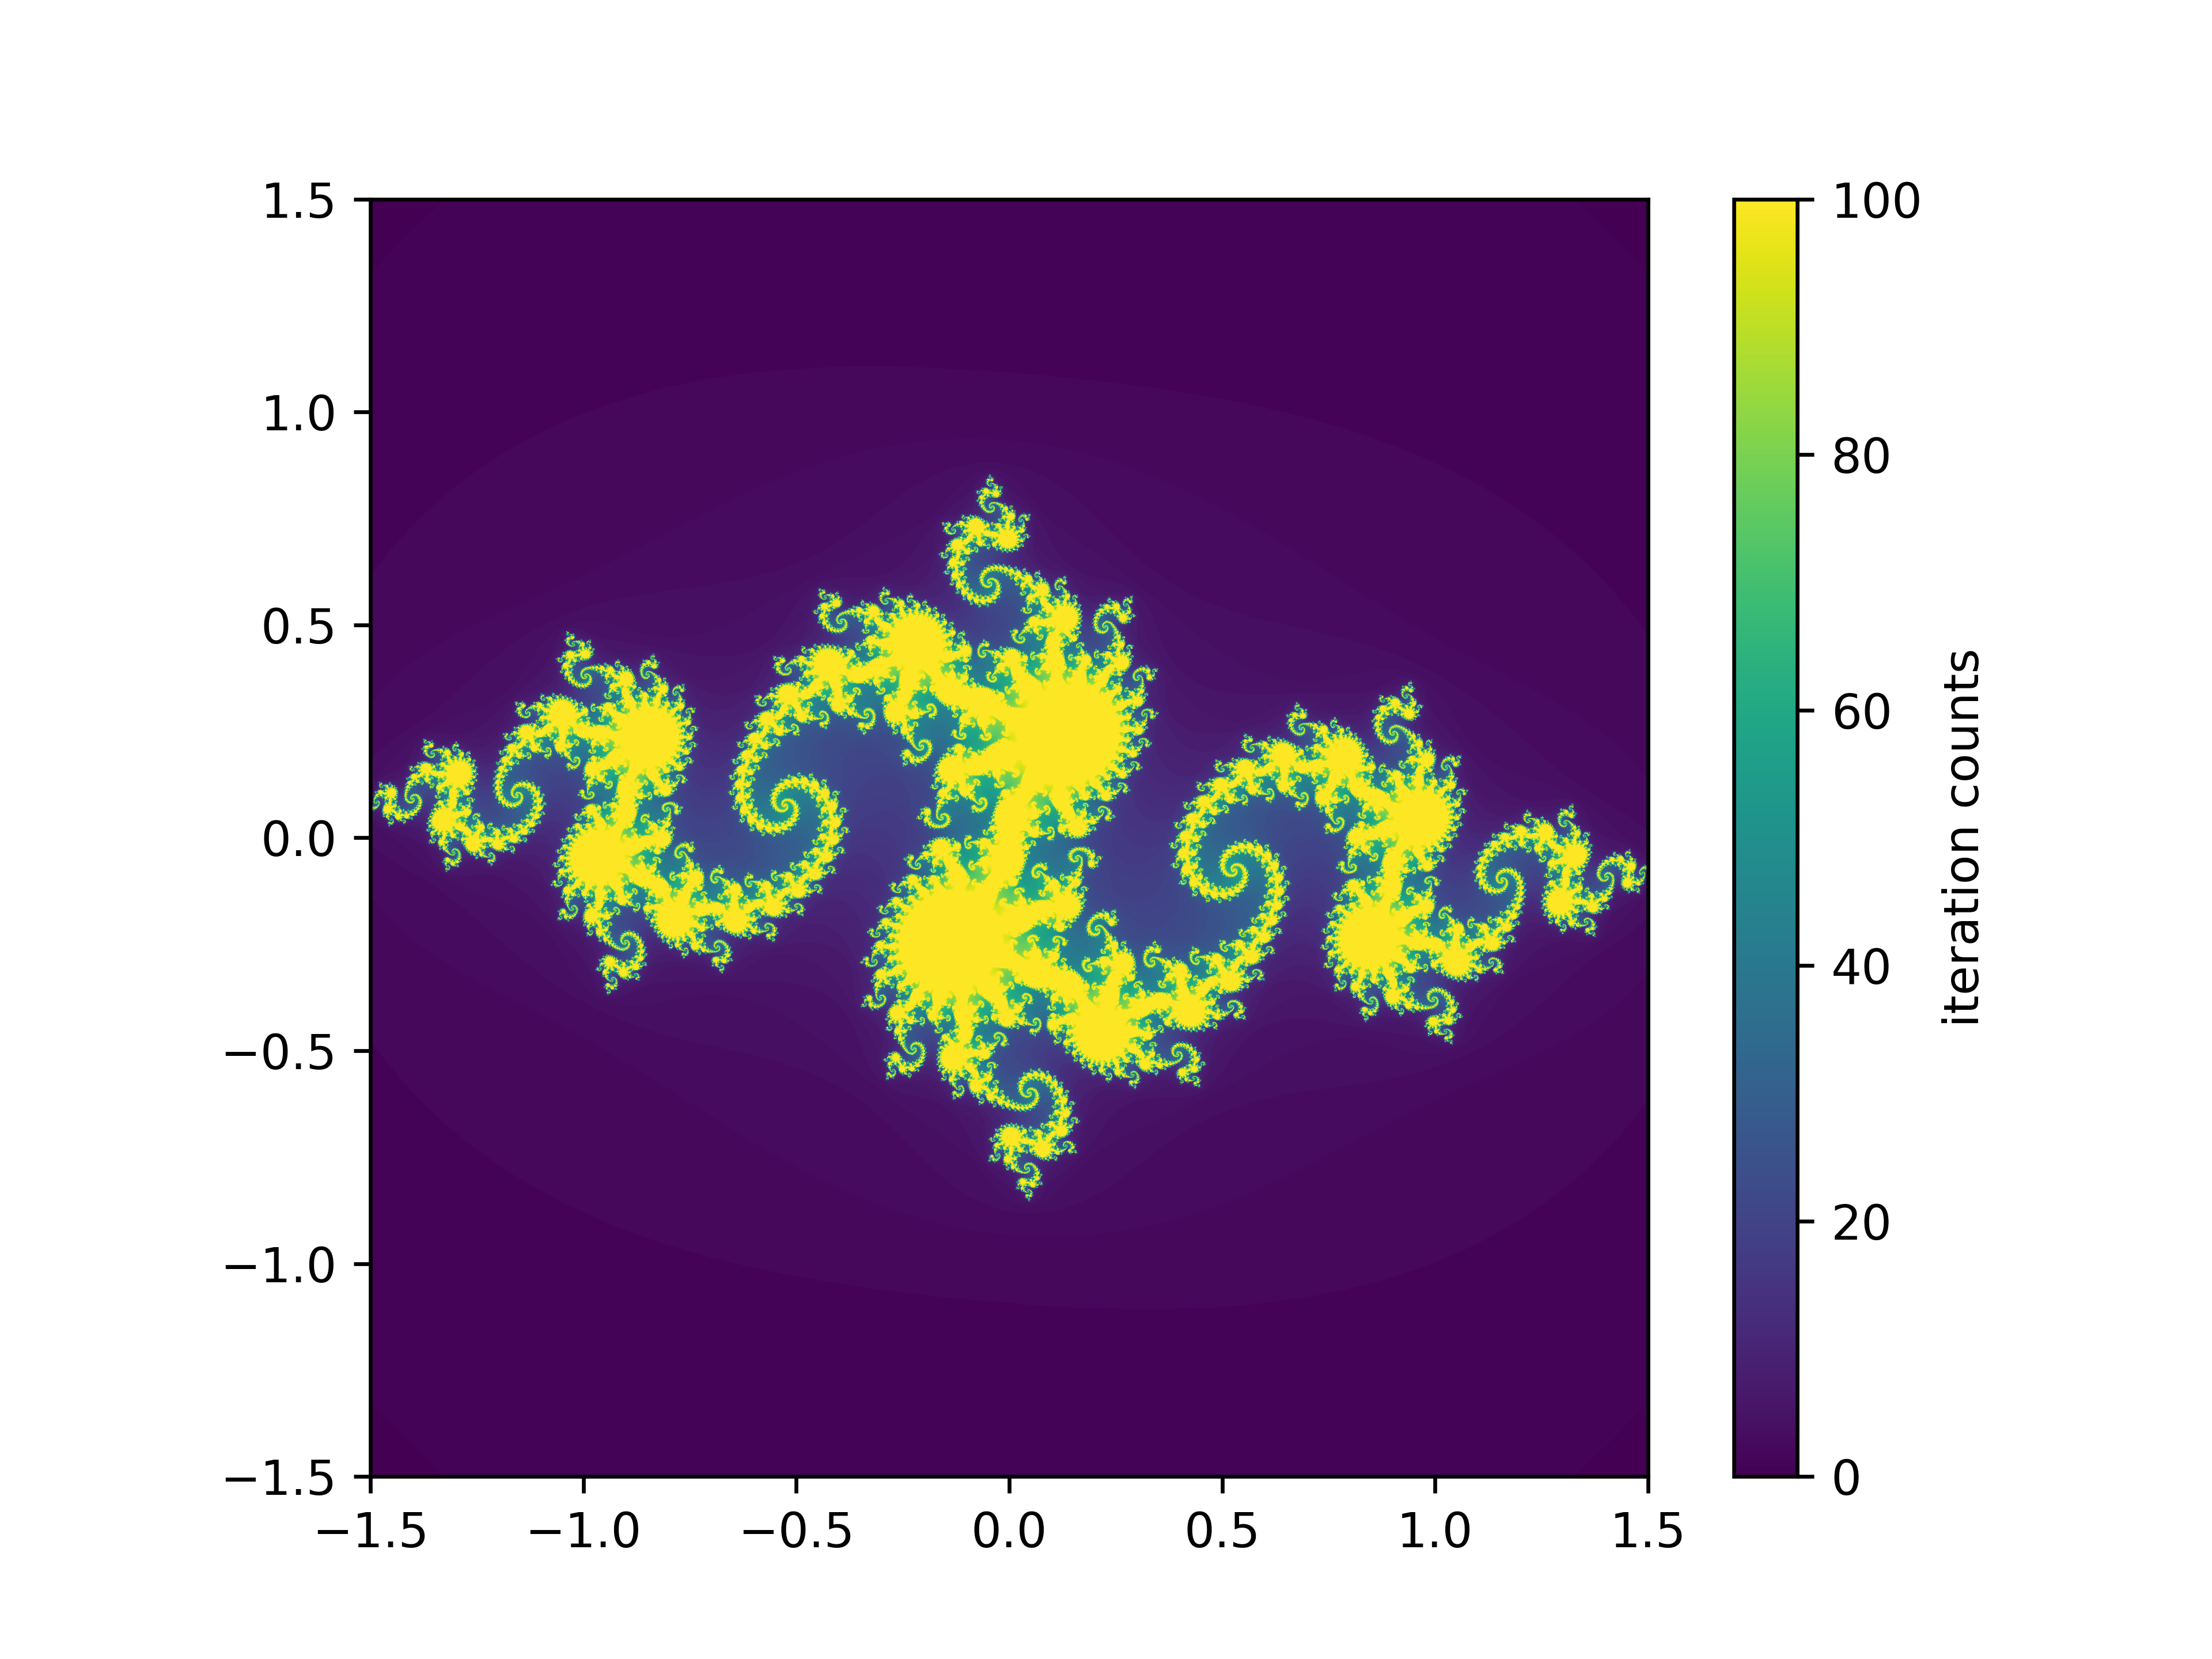
\includegraphics[width=.45\textwidth]{./png/300dpi/julia_cx-0.8cy0.156_N100.png}
	\caption{$N=100,c=c_1,c_2,c_3,c_4$}
	\label{tu3}
\end{figure}

\subsection{改变迭代公式$f(z)$}
取$N=100$,令$f_1(z)=z^3-0.071-1.134i$,$\displaystyle f_2(z)=\frac{(1-\frac{z^3}{6})}{(z-\frac{z^2}{2})^2}-0.616+0.45i$\cite{julia_wiki},如图\ref{tu4}所示。可以观察的到,即使$f(z)$改变了,生成的Julia集的图像仍然具有分形的性质,在这之中体现出了数学之美。
\begin{figure}[H]
	\centering
	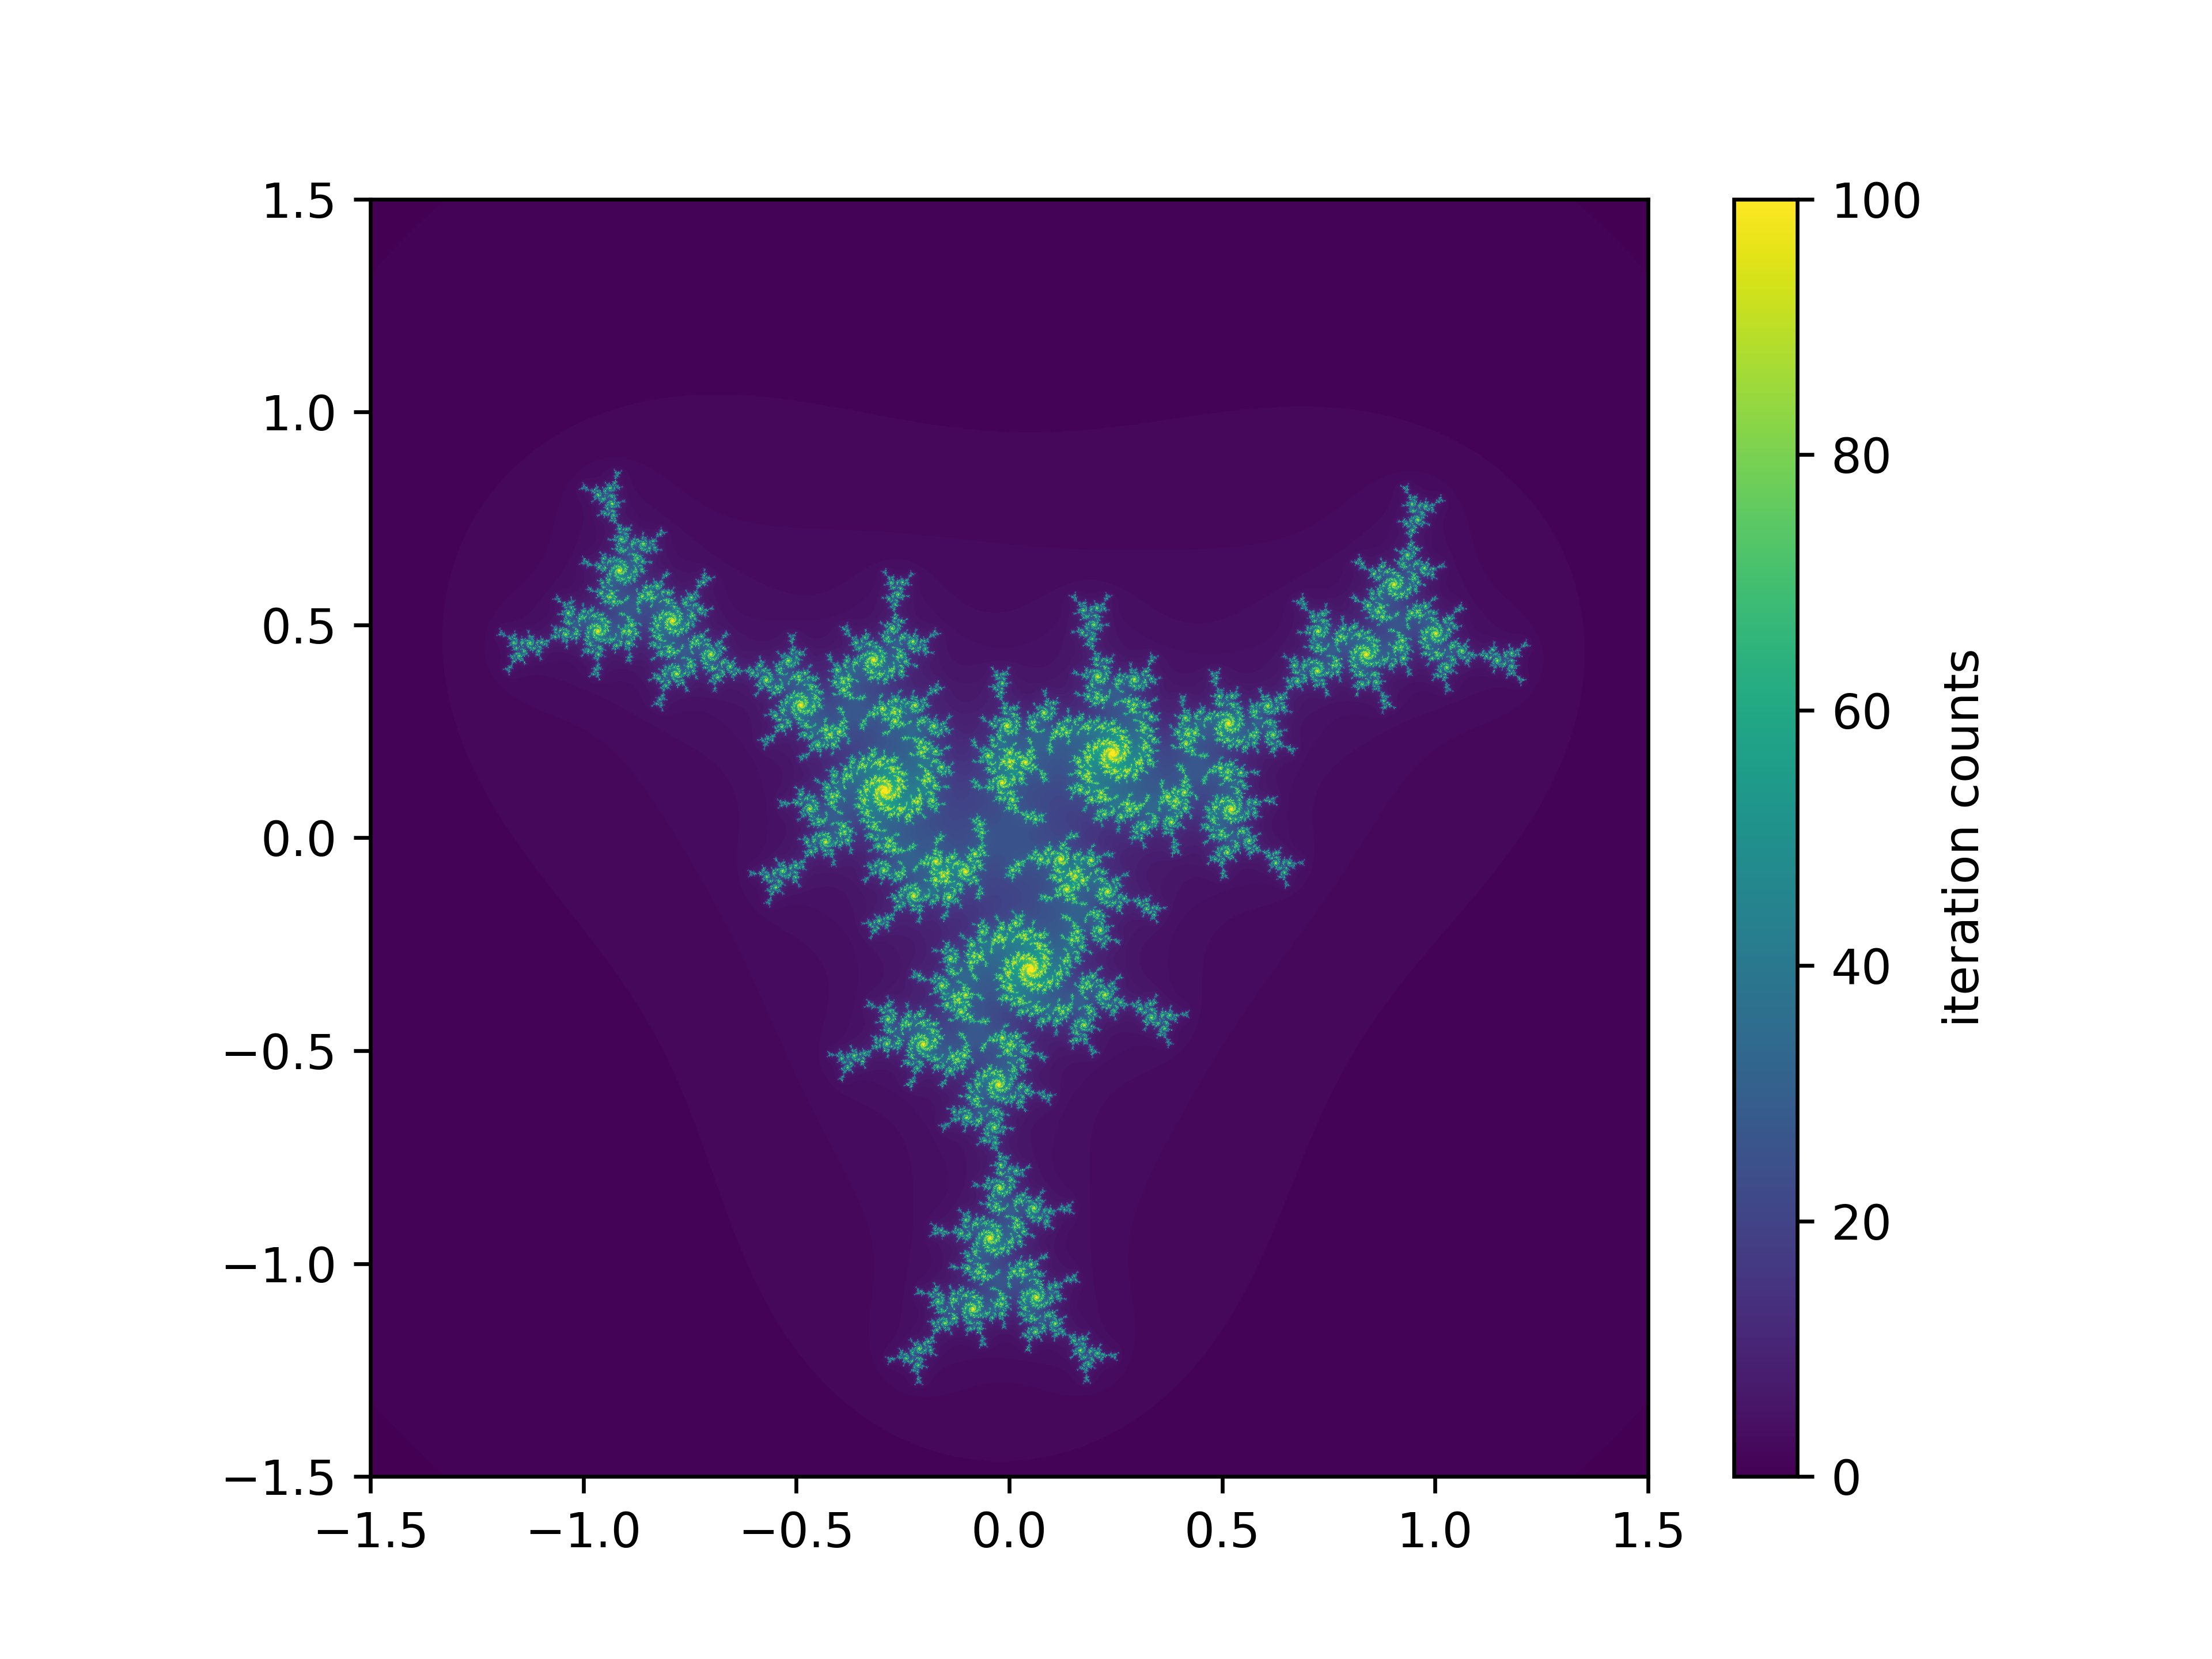
\includegraphics[width=.45\textwidth]{./png/300dpi/julia_f1_N100.png}
	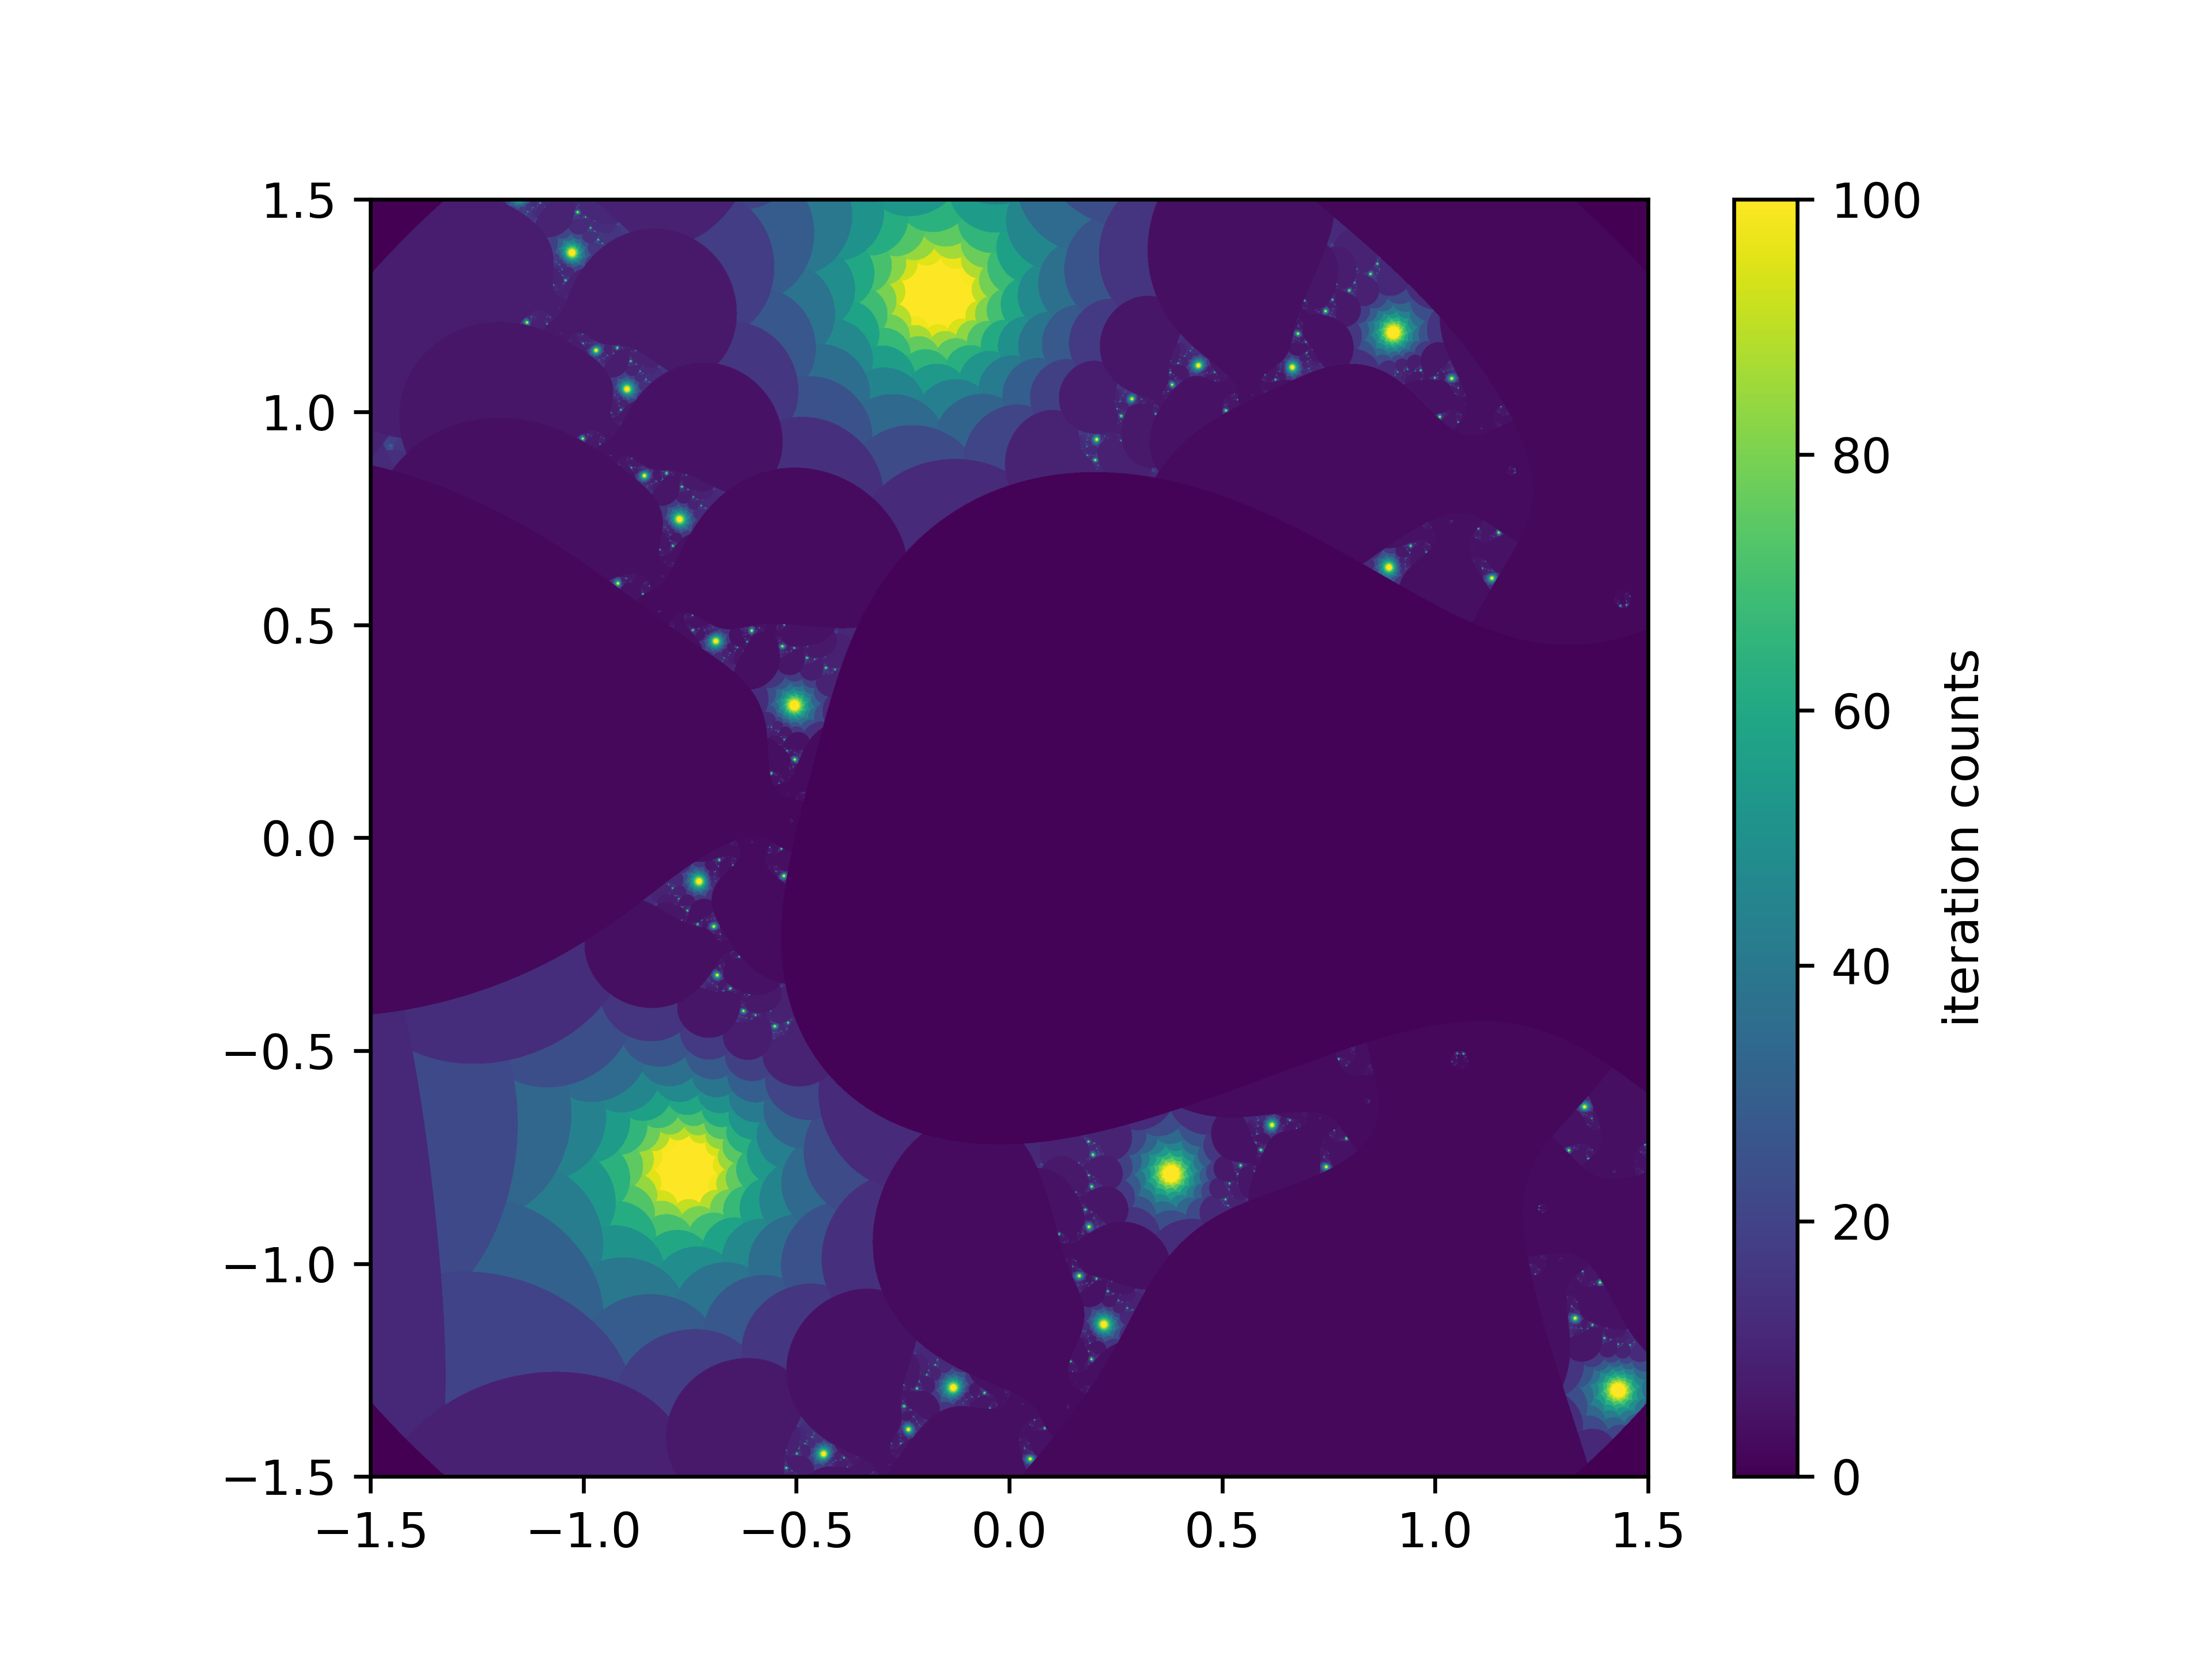
\includegraphics[width=.45\textwidth]{./png/300dpi/julia_f2_N100.png}
	\caption{$N=100,f(z)=f_1(z),f_2(z)$}
	\label{tu4}
\end{figure}

\section{拓展:Julia集和Mandelbrot集之间的关系}
实际上Julia集和Mandelbrot集就是同一函数$f(z)$对不同参数的递归过程,Julia集是固定复常数$c$,取遍复数$z$进行递归,而Mandelbrot集则是固定递归初值$z_0$取遍复数$c$进行递归。而且更深入的来看,Mandelbrot集就是对Julia集的一个概括\cite{julia_zhihuRe},这是因为在Mandelbrot集中所选取的$c$值对应到Julia集时,这个Julia集是连通的,反之亦然。\cite{julia_Ju}

这里在src目录下提供了一个python代码\texttt{man\_julia.py}\cite{julia_zhihuRe},运行后可以得到一个窗口(如图\ref{tu5}所示),点击左侧的Mandelbrot集的图像的某个点$c$的位置即可在右侧生成相应的Julia集的图像。可在根目录终端下执行命令\texttt{make relation}得到。
\begin{figure}[H]
	\centering
	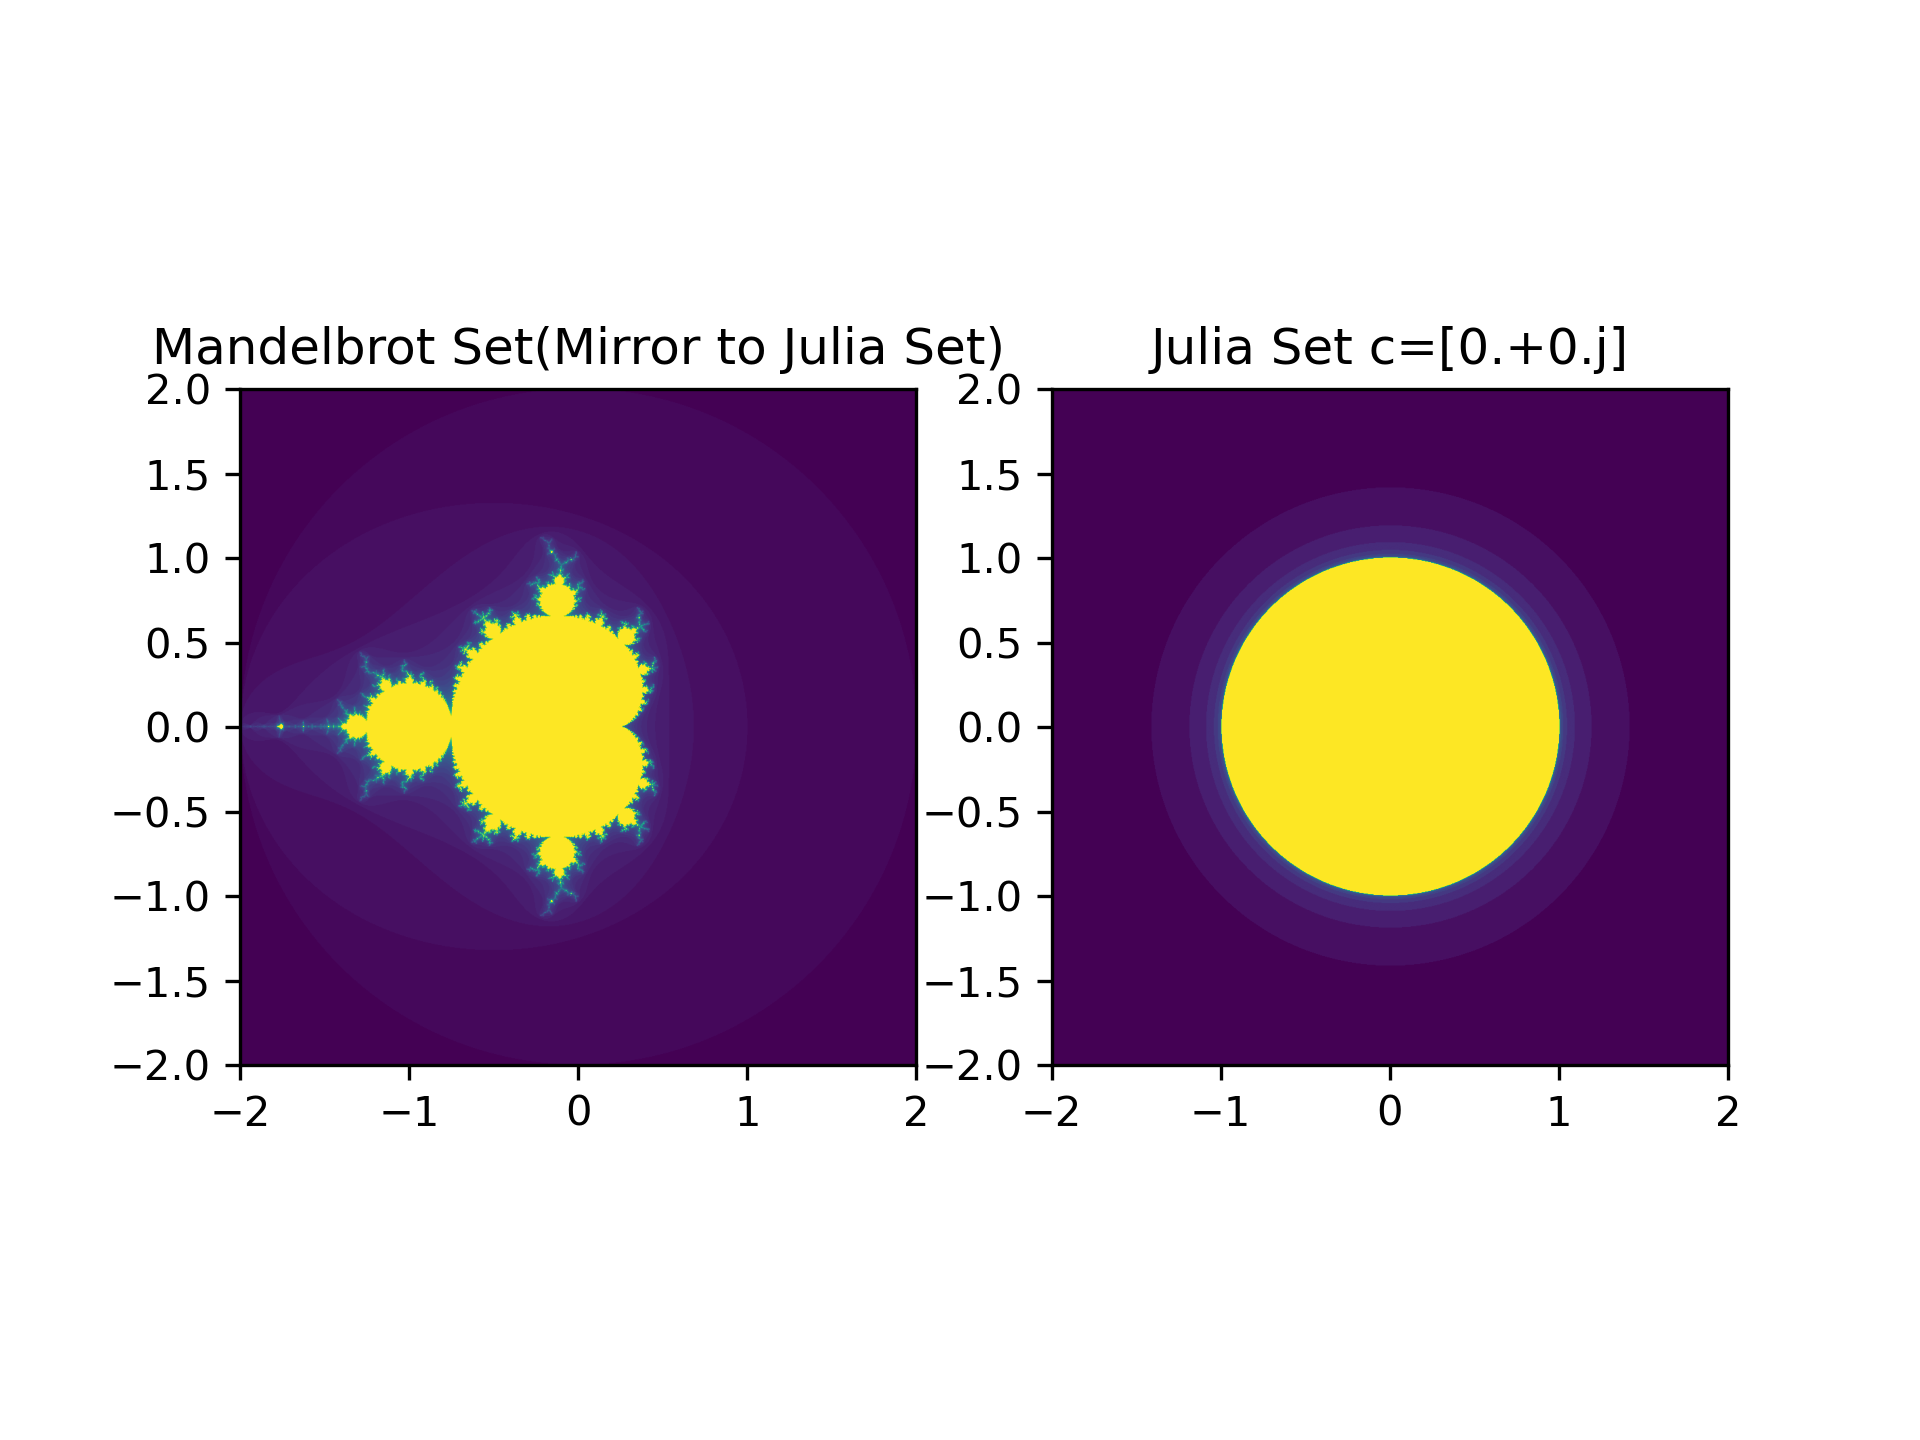
\includegraphics[width=.8\textwidth]{./png/300dpi/show.png}
	\caption{代码经ipython3运行后窗口展示}
	\label{tu5}
\end{figure}

\section{总结与思考}
通过以上简单的分析与探索,我对Julia集的性质与特征有了更深入的了解,并且通过Python语言仿照编写了程序对分析和探索的过程进行了可视化,使得这一过程更为清晰自然。于此同时,还对Mandelbrot集与Julia集的关系进行了浅显的分析与观察,而这一联系方法想必能够适用于其他的$f(z)$,这将帮助我们寻找不同$f(z)$下更能凸显图像性质的$c$值。

\centering
\bibliographystyle{plain}
\bibliography{julia.bib}	

\end{document}
